%%%%%%%%%%%%%%%%%%%%%%%%%%%%%%%%%%%%%%%%%%%%%%%%%%%%%%%%%%%%%%%%%%%%%%%%%%%%%%%%
\documentclass[english]{cgsthesis}
\usepackage[utf8]{inputenc}

% Bibtex %%%%%%%%%%%%%%%%%%%%%%%%%%%%%%%%%%%%%%%%%%%%%%%%%%%%%%%%%%%%%%%%%%%%%%%
\usepackage[defernumbers=true,natbib=true,bibencoding=ascii,backend=bibtex,style=numeric]{biblatex}
\DeclareBibliographyCategory{cited}
\DeclareBibliographyCategory{supplementary}
\AtEveryCitekey{\addtocategory{cited}{\thefield{entrykey}}}
\newcommand{\citesupplementary}[1]{\nocite{#1}\addtocategory{supplementary}{#1}}
\DefineBibliographyStrings{english}{
  andothers = {\emph{et~al.}}
}
\addbibresource{schoedon.bib}

% Code listings %%%%%%%%%%%%%%%%%%%%%%%%%%%%%%%%%%%%%%%%%%%%%%%%%%%%%%%%%%%%%%%%
\usepackage{listings}
\lstloadlanguages{C++, HTML, sh}
\lstdefinelanguage{JavaScript}{
  keywords={typeof, new, true, false, catch,%
    function, return, null, catch, switch, var,%
    if, in, while, do, else, case, break},
  ndkeywords={class, export, boolean, throw, implements, import, this},
  sensitive=false,
  comment=[l]{//},
  morecomment=[s]{/*}{*/},
  morestring=[b]',
  morestring=[b]"
}
\newcommand{\lstsetjavascript}{
  \lstset{
        language=JavaScript,
        breaklines=true,
        commentstyle=\textit,
        basicstyle=\ttfamily,
        keywordstyle=\bfseries,
        stringstyle=\ttfamily,
        showstringspaces=false,
        frame=single,
        tabsize=2
  }
}
\usepackage{glsl}

% Thesis development
\usepackage{cgsnotes}
\usepackage{cgsparagraphclassification}

% Title page
\logo{img/logo_black}

\title{{\huge Network-based Accessibility Maps}\\[-2mm] {\huge for Web Applications and Mobile Devices}}
%\title{Network-based Visualization and Interactive Rendering of Accessibility Maps for Mobile Devices and Web Applications}
%\subtitle{Netzwerkbasierte Erreichbarkeitskarten\\ für Web-Anwendungen und mobile Ger\"ate}
%\subtitle{Netzwerkbasierte Visualisierung und interaktives Rendering von Erreichbarkeitskarten in mobilen und Web-Anwendungen}

\subject{
    Master's thesis for obtaining the academic degree\\[1em]
    \enquote{Master of Science} (M.Sc.)\\[1em]
    in Geoinformation and Visualization\\
    at the chair of Computer Graphics Systems,\\
    Hasso-Plattner-Institute, University of Potsdam, Germany
    \vfill
    submitted by}
\author{Alexander Schoedon, B.Sc.}

\publishers{%
    Advisors:\\
    Prof.\ Dr.\ J\"urgen D\"ollner\\
    Dr. Matthias Trapp}

\place{Potsdam}
\date{\today}

%\renewcommand*{\listlistingname}{List of XYZ}
\renewcommand{\lstlistlistingname}{List of Listings}

%%%%%%%%%%%%%%%%%%%%%%%%%%%%%%%%%%%%%%%%%%%%%%%%%%%%%%%%%%%%%%%%%%%%%%%%%%%%%%%%
\begin{document}
\frontmatter
\maketitle

%%%%%%%%%%%%%%%%%%%%%%%%%%%%%%%%%%%%%%%%%%%%%%%%%%%%%%%%%%%%%%%%%%%%%%%%%%%%%%%%
%\addchap{Sandbox}
%
%This is really early work. It is important to test the powerful tools provided by the \texttt{cgsthesis} class.\par
%\vfill
%
%Let's test low priority in-line to-dos.\lowinlinetodo{Testing low priority in-line to-dos.}
%Let's test medium priority in-line to-dos.\mediuminlinetodo{Testing medium priority in-line to-dos.}
%Let's test high priority in-line to-dos.\highinlinetodo{Testing high priority in-line to-dos.}
%Let's test massive priority in-line to-dos.\massiveinlinetodo{Testing massive priority in-line to-dos.}
%Let's test blocking priority in-line to-dos.\blockinginlinetodo{Testing blocking priority in-line to-dos.}
%\vfill
%
%\pprelim
%This is a preliminary drafted text, please work on this.\par
%\pfeedback
%This is a to-be-reviewed text, get feedback on that version.\par
%\pfinal
%This is a final, multiple times reviewed version, submit it.\par
%\vfill
%\lowinlinetodo{Remove the sandbox page.}

%\addchap{Roadmap}
%\begin{itemize}
%\itemsep-0.7em
%\item[\textbf{04} ~ ~ ~ ~ ~] \textbf{April}
%\item[15.04 . . . . ] Camera Ready Copy: Short Paper EuroVis 2016
%\item[22.04 . . . . ] Master's Thesis: Road map, Table of Contents
%\item[29.04 . . . . ] Specification: White paper Back end
%\item[ ]              ~
%\item[\textbf{05} ~ ~ ~ ~ ~] \textbf{May}
%\item[07.05 . . . . ] Code: Proof-of-Concept \#5 (WebGL Tiling)
%\item[13.05 . . . . ] Code: Proof-of-Concept \#5 (WebGL Tiling)
%\item[20.05 . . . . ] Draft: Short Paper Presentation EuroVis 2016
%\item[27.05 . . . . ] Code: Proof-of-Concept \#5 (WebGL Tiling)
%\item[ ]              ~
%\item[\textbf{06} ~ ~ ~ ~ ~] \textbf{June}
%\item[03.06 . . . . ] Revise: Short Paper Presentation EuroVis 2016
%\item[10.06 . . . . ] Conference: EuroVis 2016 Groningen
%\item[17.06 . . . . ] Code: Proof-of-Concept \#6 (glTF Tiling)
%\item[24.06 . . . . ] Code: Proof-of-Concept \#6 (glTF Tiling)
%\item[ ]              ~
%\item[\textbf{07} ~ ~ ~ ~ ~] \textbf{July}
%\item[01.07 . . . . ] Code: Proof-of-Concept \#6 (glTF Tiling)
%\item[08.07 . . . . ] Thesis: Write Chapter \#5 (Web-based proof-of-concept)
%\item[15.07 . . . . ] Thesis: Write Chapter \#4 (Conception of the technique)
%\item[22.07 . . . . ] Thesis: Write Chapter \#3 (Requirements for the technique)
%\item[29.07 . . . . ] Thesis: Write Chapter \#6 (Application examples and evaluation)
%\item[ ]              ~
%\item[\textbf{08} ~ ~ ~ ~ ~] \textbf{August}
%\item[05.08 . . . . ] Thesis: Write Chapter \#7 (Discussion of the results)
%\item[12.08 . . . . ] Thesis: Write Chapter \#2 (Overview and related work)
%\item[19.08 . . . . ] Thesis: Write Chapter \#1 (Introduction)
%\item[26.08 . . . . ] Thesis: Write Chapter \#8 (Conclusion)
%\item[ ]              ~
%\item[\textbf{09} ~ ~ ~ ~ ~] \textbf{September}
%\item[02.09 . . . . ] Thesis: First Review Copy
%\item[09.09 . . . . ] Review: Feedback Loop \#1
%\item[16.09 . . . . ] Review: Feedback Loop \#2
%\item[23.09 . . . . ] \textit{(Conference)}
%\item[30.09 . . . . ] Review: Layout \& Final Setting
%\item[ ]              ~
%\item[\textbf{10} ~ ~ ~ ~ ~] \textbf{October}
%\item[07.10 . . . . ] \textit{(Hackathon)}
%\item[14.10 . . . . ] \textit{(Hackathon)}
%\item[21.10 . . . . ] \textit{(Hackathon)}
%\item[28.10 . . . . ] \textit{(Hackathon)}
%\item[\textbf{11} ~ ~ ~ ~ ~] \textbf{November}
%\item[04.11 . . . . ] Camera Ready Copy: Master's Thesis
%\end{itemize}
%~ \vfill
%\lowinlinetodo{Remove the roadmap from document.}
%Title page: Check if CGS header is available in English.\lowinlinetodo{Check if CGS header is available in English.}
%Table of Contents: Add nomenclature\mediuminlinetodo{Add nomenclature to document.}
%%%%%%%%%%%%%%%%%%%%%%%%%%%%%%%%%%%%%%%%%%%%%%%%%%%%%%%%%%%%%%%%%%%%%%%%%%%%%%%%

%%%%%%%%%%%%%%%%%%%%%%%%%%%%%%%%%%%%%%%%%%%%%%%%%%%%%%%%%%%%%%%%%%%%%%%%%%%%%%%%
\cleardoublepage              %%% Abstract                                   %%%
\addchap{Abstract}

%\pfeedback
Accessibility is a fundamental aspect in transportation, routing, and spare-time activity planning concerning traveling in modern cities. In this context, interactive web-based accessibility-map visualization techniques and systems are important tools for provisioning, exploration, analysis, and assessment of multi-modal and location-based travel time data and routing information. To enable their effective application, such interactive visualization techniques  demands for flexible mappings with respect to user-adjustable parameters such as maximum travel times, the types of transportation used, or displayed color schemes. However, traditional approaches for web-based visualization of transportation networks do not allow this degree of parametrization without significant latencies introduced by required data processing and transmission between the routing server and the visualization client. This thesis presents a novel web-based visualization technique that allows for efficient client-side mapping and rendering of accessibility data onto complex transportation networks using WebGL and glTF. A performance evaluation and comparison shows the superior performance of the approach over alternative implementations.\\[1em]

%\pprelim
%\textit{Die Erreichbarkeit ist ein wesentlicher Aspekt in Transport, Routing und Freizeitaktivitätenplanung in Bezug auf in modernen Städten reisen. In diesem Zusammenhang, interaktive Web-basierte Zugänglichkeit-Karte Visualisierungstechniken und Systeme sind wichtige Werkzeuge für die Bereitstellung, Exploration, Analyse und Bewertung von multimodalen und standortbasierte Reisezeitdaten und Routing-Informationen. Um ihre effektive Anwendung, wie interaktive Visualisierungstechniken Anforderungen für flexible Zuordnungen in Bezug auf vom Benutzer einstellbare Parameter wie maximale Fahrzeiten ermöglichen, die Art von Transport, oder Farbschemata verwendet. Allerdings traditionelle Ansätze für die webbasierte Visualisierung der Zugänglichkeit-Karten erlauben nicht dieses Maß an Parametrisierung ohne signifikante Verzögerungen durch erforderliche Datenverarbeitung und Übertragung zwischen dem Routing-Server und dem Client Visualisierung eingeführt. Dieser Beitrag stellt eine neuartige webbasierte Visualisierungstechnik, die für eine effiziente Client-seitige Abbildung und Rendering der Zugänglichkeit von Daten auf Transportnetze mit WebGL und die OpenGL-Übertragungsformat ermöglicht. Eine Leistungsbewertung und der Vergleich zeigt die überlegene Leistung der Ansatz über alternative Implementierungen.}%\mediuminlinetodo{Translate abstract to German. Avoid Google Translate ;-)}
%%%%%%%%%%%%%%%%%%%%%%%%%%%%%%%%%%%%%%%%%%%%%%%%%%%%%%%%%%%%%%%%%%%%%%%%%%%%%%%%


%%%%%%%%%%%%%%%%%%%%%%%%%%%%%%%%%%%%%%%%%%%%%%%%%%%%%%%%%%%%%%%%%%%%%%%%%%%%%%%%
\cleardoublepage              %%% TABLE OF CONTENTS                          %%%
\phantomsection
\addcontentsline{toc}{chapter}{Table of Contents}
\tableofcontents
%%%%%%%%%%%%%%%%%%%%%%%%%%%%%%%%%%%%%%%%%%%%%%%%%%%%%%%%%%%%%%%%%%%%%%%%%%%%%%%%

%%%%%%%%%%%%%%%%%%%%%%%%%%%%%%%%%%%%%%%%%%%%%%%%%%%%%%%%%%%%%%%%%%%%%%%%%%%%%%%%
\cleardoublepage              %%% LIST OF FIGURES                            %%%
\listoffigures
%%%%%%%%%%%%%%%%%%%%%%%%%%%%%%%%%%%%%%%%%%%%%%%%%%%%%%%%%%%%%%%%%%%%%%%%%%%%%%%%

%%%%%%%%%%%%%%%%%%%%%%%%%%%%%%%%%%%%%%%%%%%%%%%%%%%%%%%%%%%%%%%%%%%%%%%%%%%%%%%%
\cleardoublepage              %%% LIST OF TABLES                             %%%
\listoftables
%%%%%%%%%%%%%%%%%%%%%%%%%%%%%%%%%%%%%%%%%%%%%%%%%%%%%%%%%%%%%%%%%%%%%%%%%%%%%%%%

%%%%%%%%%%%%%%%%%%%%%%%%%%%%%%%%%%%%%%%%%%%%%%%%%%%%%%%%%%%%%%%%%%%%%%%%%%%%%%%%
\cleardoublepage              %%% LIST OF LISTINGS                           %%%
\lstlistoflistings % @TODO list of listings
%%%%%%%%%%%%%%%%%%%%%%%%%%%%%%%%%%%%%%%%%%%%%%%%%%%%%%%%%%%%%%%%%%%%%%%%%%%%%%%%

\mainmatter

%!TEX root = ../schoedon.tex


\cleardoublepage
\chapter{Introduction}
  \label{chap:intro}
  This thesis proposes a new technique for web-based transportation network
  visualizations within the application of network-based accessibility maps.\par

  \section{Motivation}
    \label{sec:intro:motiv}
    Different approaches for rendering maps in web applications exist.
    Widely used architectures are raster or vector services that provide web
    mapping applications with geographic data in client/server models.
    Raster data is efficiently mapped and rendered server-side using a
    static, predefined display. Vector data can be rendered client-side
    using dynamic mappings and interactive stylization.\par

    \begin{figure}[htb]
      \centering
      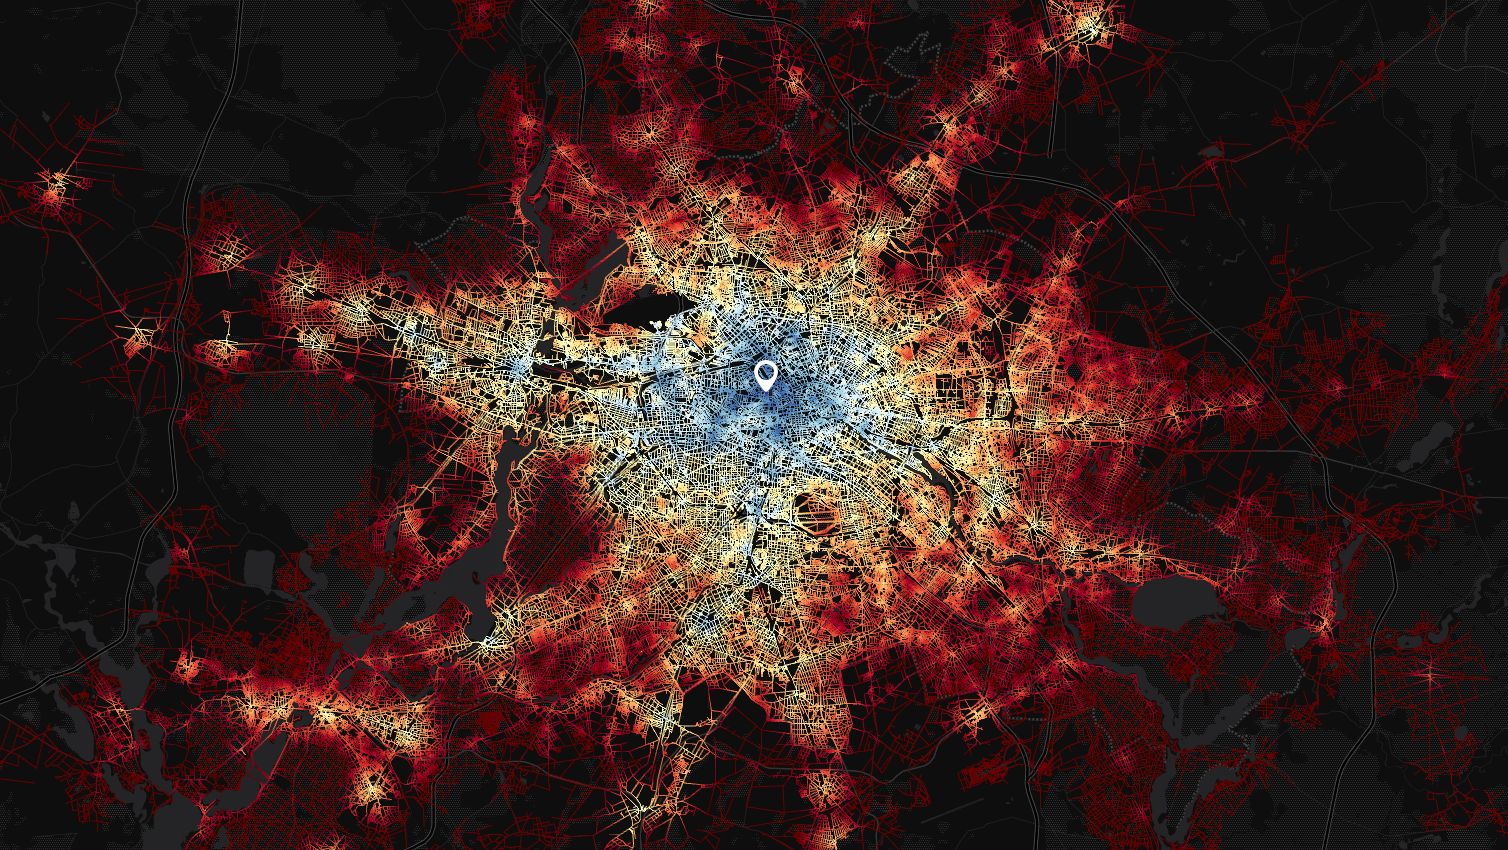
\includegraphics[width=\linewidth]
        {./img/screenshot-teaser-7200s-publictransport.png}
      \caption{A network-based accessibility map visualization.}
      \label{fig:intro:teasr}
    \end{figure}

    However, these techniques do not supply a convenient approach to map and
    render high detailed, unfiltered transportation network geometries
    required for applications such as accessibility analytics (compare Figure
    \ref{fig:intro:teasr}).\par

  \section{Definitions}
    \label{sec:intro:def}

    Both the terms \textit{transportation networks} and \textit{accessibility
    maps} are ambiguous and will be defined for future usage in this
    thesis.\par

    \begin{description}
      \item[Transportation Network] is a routable graph representation of a
        geographic dataset.
        It includes all types of roads from motorways to residential paths
        including foot-ways and cycle-ways [??]. It does not include railways or
        bus guide-ways which are not accessible by private means of transport.
      \item[Accessibility Maps] are a tool for mobility analytics. They display
        single source shortest path (\acrshort{sssp}) routing for selected
        geographic areas [??]. Accessibility can used be as a synonym for
        \textit{reachability} in this case. It's not related to services or
        environments for people who experience disabilities.

        % reachability analysis in Innerebner (2013)
        % travel time maps in Campenhout (2010)
        % both Yin (2015)

    \end{description}

  \section{Problem statement}
    \label{sec:intro:probl}

    Figure \ref{fig:intro:r360d} shows an existing web service for accessibility
    mapping. It encodes travel time intervals using separate polygons, which
    must be computed and transferred to the browser. This kind of approach has
    several drawbacks:\par

    \begin{enumerate}[\label=({D}1)]
      \item It's creation requires generalization.
      \item It lacks precision with regard to the network.
      \item It does not scale for a more detailed display.
    \end{enumerate}

    \begin{figure}[htb]
      \centering
      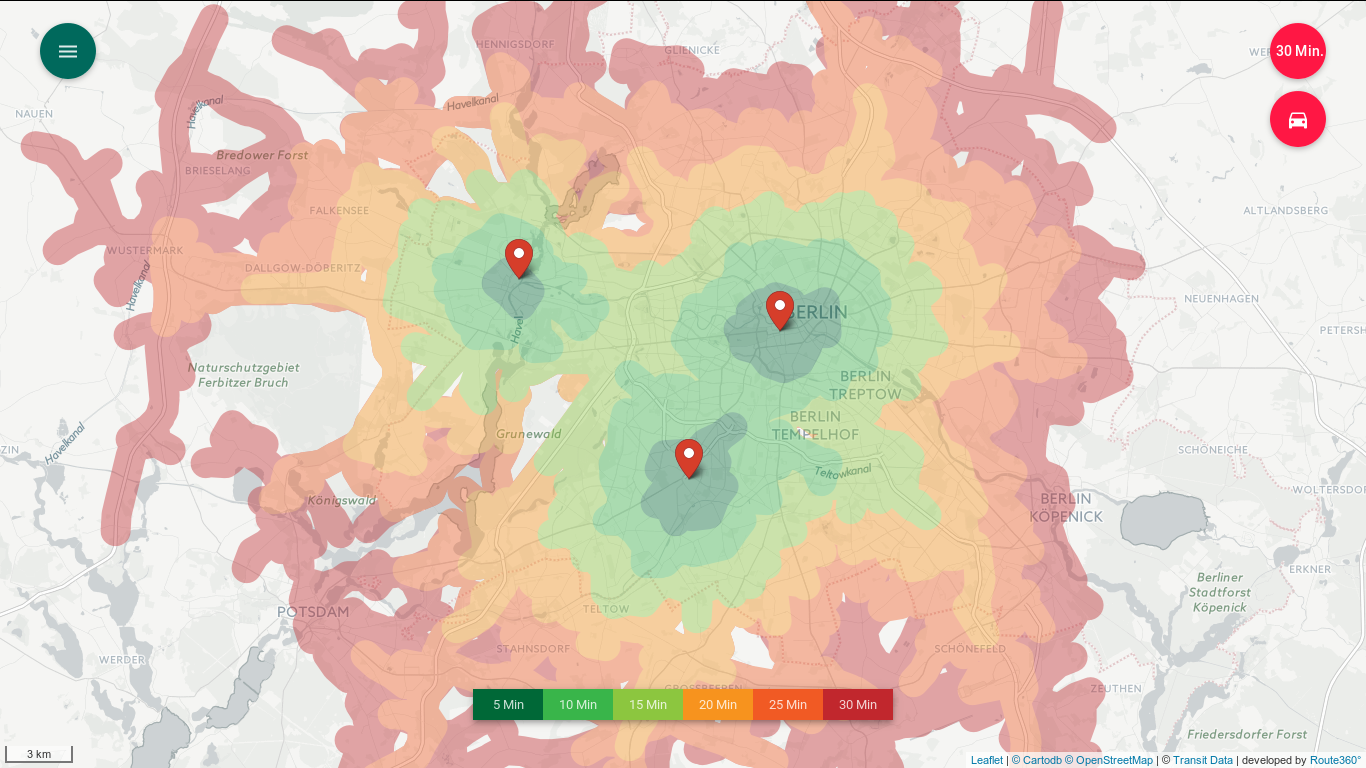
\includegraphics[width=\linewidth]
        {./img/screenshot-r360js-demo.png}
      \caption{A generalized, polygon-based accessibility map visualization
        by Motion Intelligence GmbH utilizing the Route360$^\circ$-\acrshort{js}
        \acrshort{api} [??].}
      \label{fig:intro:r360d}
    \end{figure}

    Real-time rendering transportation networks as scenery for data
    visualization in web-based applications is a performance critical task
    depending on the geometric complexity of the network and associated travel
    times. For example, an OpenStreetMap (\acrshort{osm}) dataset of the Berlin
    region comprises approximately $2.4 \cdot 10^6$ road segments spanned by
    $2.9 \cdot 10^6$ vertices as of June 2016 [??]. Using traditional
    visualization
    approaches using web browsers either faces users with a predefined, static
    filtering and mapping (raster data) or a notable computation-intense
    rendering process (vector data). These two fundamental approaches covering
    filtering, mapping, and rendering web-based maps are widely established and
    have proven to be effective, but exhibit drawbacks.\par

    Data transmitted in pre-rendered raster data formats (e.g., \acrshort{png},
    \acrshort{jpg}) does
    not require any client-side processing prior to rendering, can be compressed
    as well as cached~\cite{ESRI2006}, and is used by major web-mapping services
    such as Google or Bing maps [??]. However, one major disadvantage is the
    lack for client-side filtering and mapping without requesting a complete map
    tile reload. Web services using this technology approach this by using small
    vector overlays displaying additional user-styled information [??], but it
    is not possible to access the the map data itself.\par

    In contrast thereto, geo-data transmitted using vector formats
    (e.g., \acrshort{json}, \acrshort{gml}) enable
    client-side filtering, mapping, and rendering. This client-side processing
    however introduces a major performance impact: both the data processing and
    rendering are usually performed on central processing units (\acrshort{cpu})
    using JavaScript (\acrshort{js}) algorithms. Recent approaches do support
    hardware-accelerated rendering (\acrshort{gpu}) but lack functionality for
    client-side vector data processing~\cite{Gaffuri2012}.\par

    Thus, both approach changes in filtering (e.g., selecting a travel time
    threshold) or mapping (e.g., color mapping, line styles etc.) would result
    in a complete data re-transmission, loading, and processing.\par

    Therefore, high detailed network analysis and visualization is often
    performed using Geographic Information Systems (\acrshort{gis}). Such
    systems
    exploit the computation power of desktop workstations but posses limited
    applicability to everyday life, due to data availability and access, as well
    as expert domain knowledge required by a user.\par

  \section{Contributions}
    \label{sec:intro:contr}

    In the light of powerful, dedicated graphics hardware being not only
    available on personal computers (\acrshort{pc}) but also
    on small, mobile devices nowadays, this thesis suggests new techniques for
    client-side rendering of web-maps with complex geometries on graphic
    processing units (\acrshort{gpu}).\par

    The challenge of this work is twofold interesting. On the one hand it is
    important to enable rendering using GPU-based techniques like
    the web graphics library (\acrshort{webgl}) \cite{Jackson2016}.
    This allows dynamic, interactive and user-defined styles to be rendered
    directly on the client's device. But on the other hand it is a must to
    completely eliminate the client-side mapping of the geo-data as this becomes
    a major performance bottleneck with increasing data complexity.\par

    This thesis proposes a new approach for web-based visualization of
    accessibility maps based on transportation network data. This geometry-based
    approach uses vector data (lines) stored and transmitted using the new
    standardized graphics library transmission format (\acrshort{gltf}) [??],
    which reduces performance-critical
    computations in the visualization client (i.e., coordinate transformations)
    and thus facilitates real-time rendering with high run-time performance
    yielding low client response times. To summarize, this work makes the
    following contributions:\par

    \begin{enumerate}[\label=({C}1)]
      \item It presents a concept to decouple the visualization geometry and
        data items for interactive web-based accessibility maps based on
        \acrshort{webgl}.
      \item It specifies a geographic tiling concept based on a binary
        transmission format close to rendering requirements
        utilizing the new standardized \acrshort{gltf}.
      \item It demonstrates the effectiveness of this approach by a
        comparative performance evaluation of different implementation
        variants.
    \end{enumerate} % @TODO compare innereber thesis 2013

    The technique presented in this thesis is a graphics library (\acrshort{gl})
    based approach rather than classic vector- or raster-based provisions.
    It shows various advantages:\par

    \begin{enumerate}[\label=({A}1)]
      \item Its usage is not limited to stationary desktop systems but available
        on a variety of devices (esp. mobile).
      \item Potentially massive data sources are not required to be completely
        transmitted, stored, or managed.
      \item Implementations based on web-services and \acrshort{webgl} can be
        easily integrated into existing systems and visualization frameworks.
    \end{enumerate}

    In contrast to existing accessibility-map visualization concepts, this work
    focuses on visualizing the travel time data directly on the respective
    transportation network features, rather than (possibility generalized)
    polygons~\cite{Glander2010} or specific graph layouts~\cite{Krause2012}.
    This enables a precise mapping of travel data to the geo-referenced
    transportation network. However, considering the high geometric complexity
    (vertices, primitives) introduced by increasing quality of transportation
    networks~\cite{Zielstra2010}, e.g., of massive open data transportation
    networks (OpenStreetMap (\acrshort{osm}) or General Transit Feed
    Specification (\acrshort{gtfs})),
    an implementation of an interactive web-based visualization technique
    comprises a number of conceptual and technical challenges.\par

    It maintains the goal to allow real-time rendering with outstanding
    performance and very low response times for the client.\par


  \section{Publications}
    \label{sec:intro:publc}
    \begin{itemize}
      \item \cite{STHD2016} \textsc{Schoedon, A; Trapp, M; Hollburg, H; Döllner, J (2016)}:\\ Interactive Web-based Visualization for Accessibility Mapping of Transportation Networks. In: Eurographics Conference on Visualization (\textsc{EuroVis}) 2016, The Eurographics Association, Groningen.
    \end{itemize}

  \section{Thesis Organization}
    \label{sec:intro:organ}
    Foo Too Doo Bar.

%!TEX root = ../schoedon.tex

\cleardoublepage
\chapter{Overview and related work}
  \label{chap:overv}

  Table \ref{tab:overv:relat} (page \pageref{tab:overv:relat}) shows a first
  overview of related graphics, applications and publications in the broad
  field of mobility analytics and accessibility mapping techniques.\par

  \begin{table}[htp]
    \tiny \centering
    \begin{tabular}{r|l|l|l}
     \textbf{Year} & \textbf{Authors} & \textbf{Contribution} & \textbf{Type} \\
     \hline
      1881 & Galton \cite{galton1881construction} & Construction of isochronic passage-charts  & Publication  \\
      1959 & Hansen \cite{hansen1959accessibility} & How accessibility shapes land use & Publication \\
      1972 & Armstrong \cite{armstrong1972network} & Network analysis of airport accessibility  & Publication  \\
      1978 & Muller \cite{muller1978mapping} & Mapping of travel times  & Publication  \\
      1981 & Sugiura \cite{Sugiura1981} & Japan travel time maps  & Graphic  \\
      1986 & Hall \cite{hall1986fastest} & Network with random time-dependent travel times  &  Publication \\
      1989 & Cauvin et al. \cite{cauvin1989cartographic} & The piezopleth maps method  & Publication  \\
      1993 & Spierkermann et al. \cite{spiekermann1993zeitkarten} & Time maps for spatial planning  & Publication  \\
      1994 & Spierkermann et al. \cite{spiekermann1994new} & Time-space maps of Europe  & Publication  \\
      1996 & Gutierrez et al. \cite{gutierrez1996accessibility} & Accessibility analysis of the European road network  & Publication  \\
      1998 & Fritz et al. \cite{fritz1998accessibility} &  Accessibility as wilderness indicator  & Publication  \\
      1998 & Juli{\~a}o \cite{juliao1998measuring} &  Measuring accessibility with \acrshort{gis} & Publication  \\
      1999 & Miller \cite{miller1999measuring} & Measuring space-time accessibility within transportation networks & Publication \\
      1999 & Spiekermann \cite{spiekermann1999visualisierung} & Visualization of railway travel times & Publication \\
      2000 & Miller et al. \cite{miller2000gis} & \acrshort{gis} for measuring space-time accessibility in transportation & Publication \\
      2000 & O'Sullivan et al. \cite{o2000using} & Using desktop \acrshort{gis} for accessibility analysis in public transport  & Publication  \\
      2001 & Ran \cite{ran2001method} &  Method of providing travel time  & Patent \\
      2001 & Handy \cite{handy2002accessibility} & Accessibility versus mobility & Publication \\
      2002 & Lovett et al. \cite{lovett2002car} & Accessibility of general practitioner services  & Publication  \\
      2003 & Altmaier et al. \cite{Altmaier2003} & Applications for inter-operable 3D geo-visualization & Publication \\
      2003 & Dailey et al. \cite{dailey2003design} &  Multi-modal transit management system & Publication  \\
      2005 & Auxhausen \cite{axhausen2005zeitkarten} & Time-maps of Switzerland  & Publication  \\
      2005 & Chronomap \cite{Chronomap} & Drive-time analysis  & Application  \\
      2005 & Karlin \cite{Karlin2005}  & London subway travel times  & Graphic \\
      2005 & McLaren \cite{McLaren2005} & Time travel with the London tube map  & Graphic  \\
      2005 & Travel Time Tube Map \cite{Carden2006} & Interactive travel time tube map  & Application  \\
      2006 & Lightfoot \cite{Lightfoot2006} & Use-cases for travel time maps  &  Publication  \\
      2006 & Pfoser et al. \cite{pfoser2006dynamic} &  Dynamic travel time maps & Publication  \\
      2006 & Rüegg \cite{Ruegg2006} & Impact of public transport on travel times  & Poster \\
      2006 & Street \cite{street2006timecontours} & Isochrone visualization to describe transport network costs  & Master's Thesis  \\
      2007 & Brabec et al. \cite{Brabec2007} & Client-based spatial web-browsing & Publication \\
      2007 & Irving \cite{Irving2007} & Use-cases for travel time maps  & Publication  \\
      2007 & Nies et al. \cite{neis2007webbasierte} & Web-based accessibility analysis  & Publication  \\
      2008 & Bauer et al. \cite{bauer2008computing} & Isochrones in multi-modal transportation networks  & Publication  \\
      2008 & Mapumental \cite{Mapumental}  &  Maps that show time & Application  \\
      2008 & Uchida et al. \cite{Uchida2008} & Travel time to major cities  & Graphic  \\
      2009 & FreeMapTools \cite{Freemaptools} & How far can I travel  & Application  \\
      2009 & Uchida et al. \cite{uchida2009agglomeration} & Measure of urban concentration  & Publication  \\
      2010 & Antrim et al. \cite{antrim2013many} & Use-cases for \acrshort{gtfs} data & Publication  \\
      2010 & Campenhout \cite{van2010travel} & Travel time maps  & Master's Thesis  \\
      2010 & Glander et al. \cite{Glander2010} & Accessibility maps to visualize quality of mobility  &  Publication \\
      2010 & Lei et al. \cite{lei2010mapping} & Mapping transit-based access  & Publication  \\
      2010 & Marciuska et al. \cite{marciuska2010determining} & determining objects within isochrones  & Publication  \\
      2010 & Müller et al. \cite{Mueller2010} & Distance transformations for accessibility mapping  &  Publication \\
      2010 & Time Maps \cite{TimeMaps} & Public transport time maps of the Netherlands & Application  \\
      2011 & Birchler \cite{birchler2011computing} & Isochrones in multi-modal public transport networks  & Bachelor's Thesis  \\
      2011 & Gemmel \cite{gemmel2012hedonic} &  Effects of walk-ability and public transit & Master's Thesis  \\
      2011 & Gamper et al. \cite{gamper2011defining} & Defining isochrones in multi-modal spatial Networks & Publication  \\
      2011 & Isochrone.ch \cite{IsochroneCh}  & Isochrones in schedule-based public transport  & Application  \\
      2011 & Li et al. \cite{li2011dynamic} & Dynamic accessibility mapping  & Publication  \\
      2011 & Söderström \cite{soderstrom2011personal} & Internet-driven maps based on time distances  & Publication  \\
      2011 & Vaaraniemi et al. \cite{Vaaraniemi2011} & Rendering of high-quality cartographic roads & Publication \\
      2012 & Byrd \cite{Byrd2012} & Visualizing urban accessibility  & Publication  \\
      2012 & Gamper et al. \cite{gamper2012scalable} & Computation of isochrones with network expiration  & Publication  \\
      2012 & Conveyal \cite{Conveyal} & Transportation - land use analysis  & Application  \\
      2012 & Hollburg et al. \cite{hollburghier} & Interactive accessibility analysis in Potsdam & Publication  \\
      2012 & Mapnificent \cite{Mapnificent}  & Web-based reachability visualization of public transport  & Application  \\
      2012 & Mertens \cite{meertens2012} & Travel Time Maps of urban areas in the Netherlands  & Graphic  \\
      2012 & Trevett \cite{Trevett2012} & 3D transmission format \acrshort{gltf} & Presentation \\
      2012 & TripTropNYC \cite{TriptropNYC} & Web-based accessibility visualization in New York  & Application  \\
      2013 & Innerebner \cite{Innerebner2013} & Isochrones in multi-modal spatial networks  & PhD Thesis  \\
      2013 & Innerebner et al. \cite{innerebner2013isoga} & Web-based geospatial reachability analysis tool  & Publication  \\
      2013 & Transit Time NYC \cite{TransitTimeNYC} & Web-based subway transit times in New York & Application \\
      2013 & Tran et al. \cite{tran2013go_sync} & Synchronizing transit data between \acrshort{gtfs} and \acrshort{osm}  & Publication  \\
      2014 & Coughlin \cite{Coughlin2014} & 3D formats for the modern web & Publication \\
      2014 & Gortana et al. \cite{gortanaisoscope} & Visualizing temporal mobility variance  & Publication  \\
      2014 & Hollburg \cite{Hollburg2014} & Interactive analysis and visualization of accessibility & Master's Thesis  \\
      2014 & Isoscope \cite{Isoscope} & Visualizing mobility with isochrone maps  & Application  \\
      2014 & Route360° \cite{Route360} & Web-based travel time analysis  & Application  \\
      2014 & Krismer et al. \cite{krismer2014incremental} & Incremental calculation of isochrones  & Publication  \\
      2014 & Voll \cite{vollerreichbarkeiten} & Accessibility analysis of the Alps  & Publication  \\
      2015 & TravelTimePlatform \cite{TravelTimePlatform} & Search and filter by time not distance  & Application  \\
      2015 & Trapp et al. \cite{Trapp2015} & Rendering transportation networks using distance fields & Publication \\
      2015 & Yin et al. \cite{Yin2015} & Web-based accessibility analysis and travel time displays  & Publication  \\
      2016 & Schoedon et al. \cite{STHD2016} & Web-based visualization of transportation networks  & Publication  \\
    \end{tabular}
    \caption{Selected related work.}
    \label{tab:overv:relat}
  \end{table}

  \section{Noteworthy publications and theses}
    \label{sec:overv:publc}

    \begin{figure}[ht]
      \subcaptionbox{
        \label{fig:overv:isopc}
        The Isochronic Passage Chart by Francis Galton, 1881
        \cite{galton1881construction}.}
      {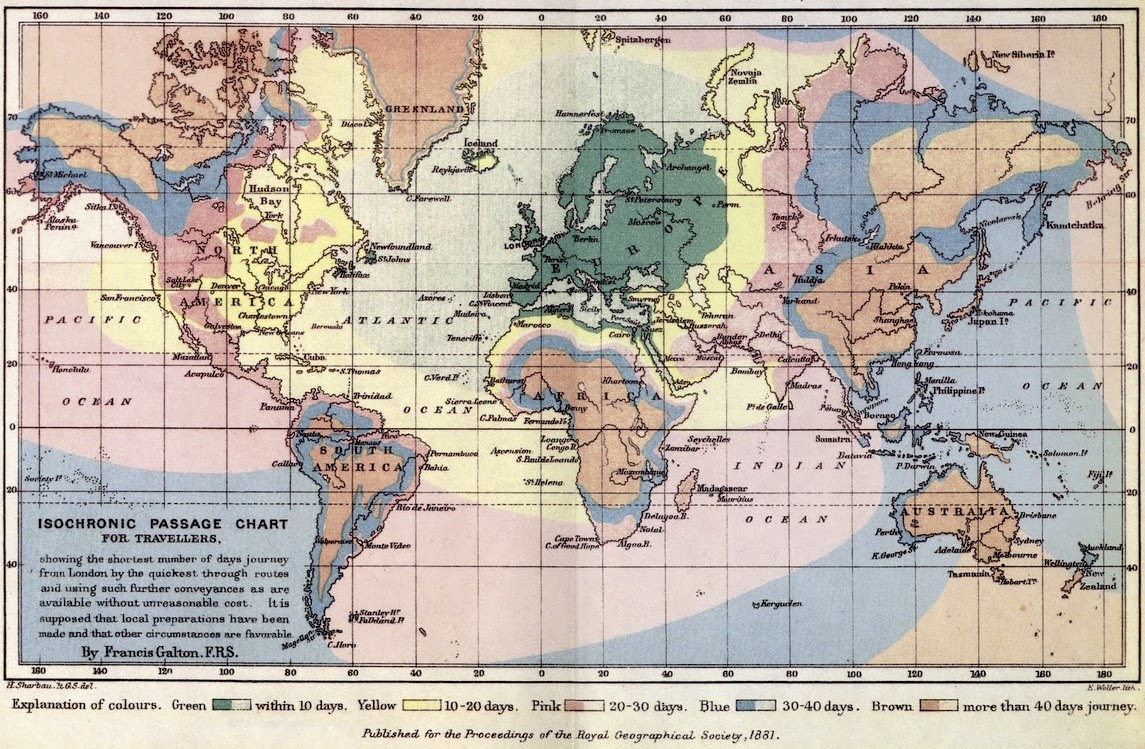
\includegraphics[width=0.32\textwidth]{./img/overv-isopc.jpg}}
      \hfill
      \subcaptionbox{
        \label{fig:overv:nodac}
        Analysis of Airport Accessibility in South Hampshire, 1972
        \cite{armstrong1972network}.}
      {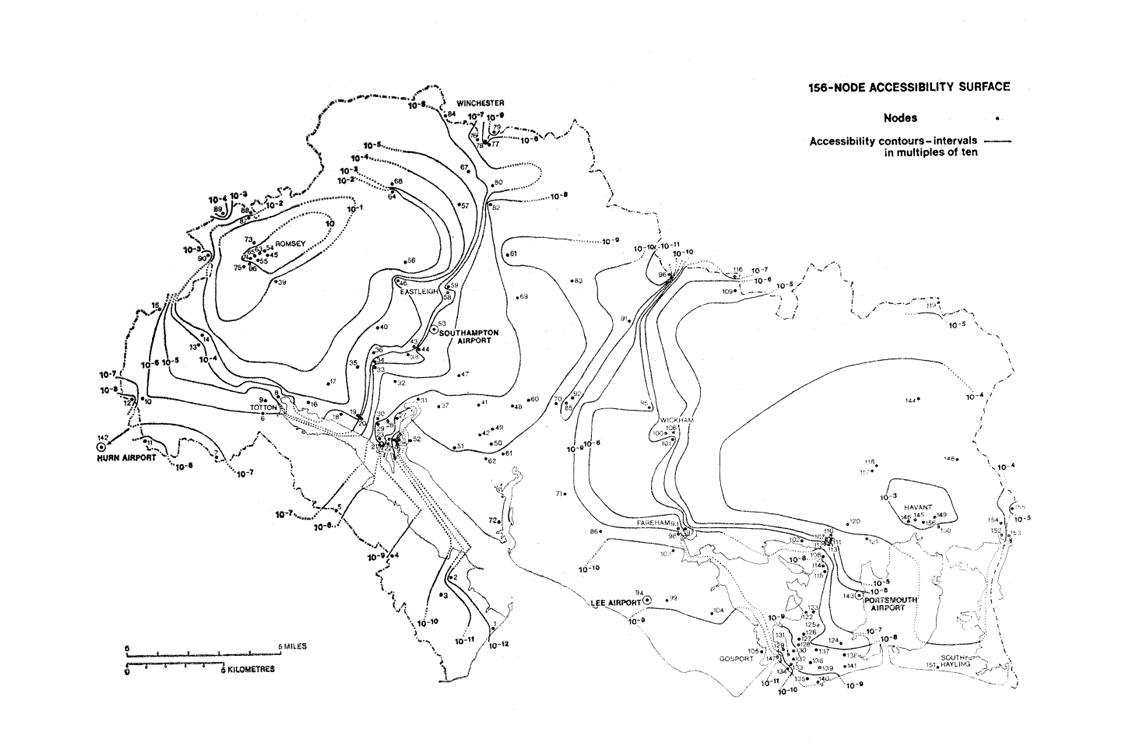
\includegraphics[width=0.32\textwidth]{./img/overv-nodac.png}}
      \hfill
      \subcaptionbox{
        \label{fig:overv:maptt}
        The Mapping of Travel Time in Edmonton, Alberta, 1978
        \cite{muller1978mapping}.}
      {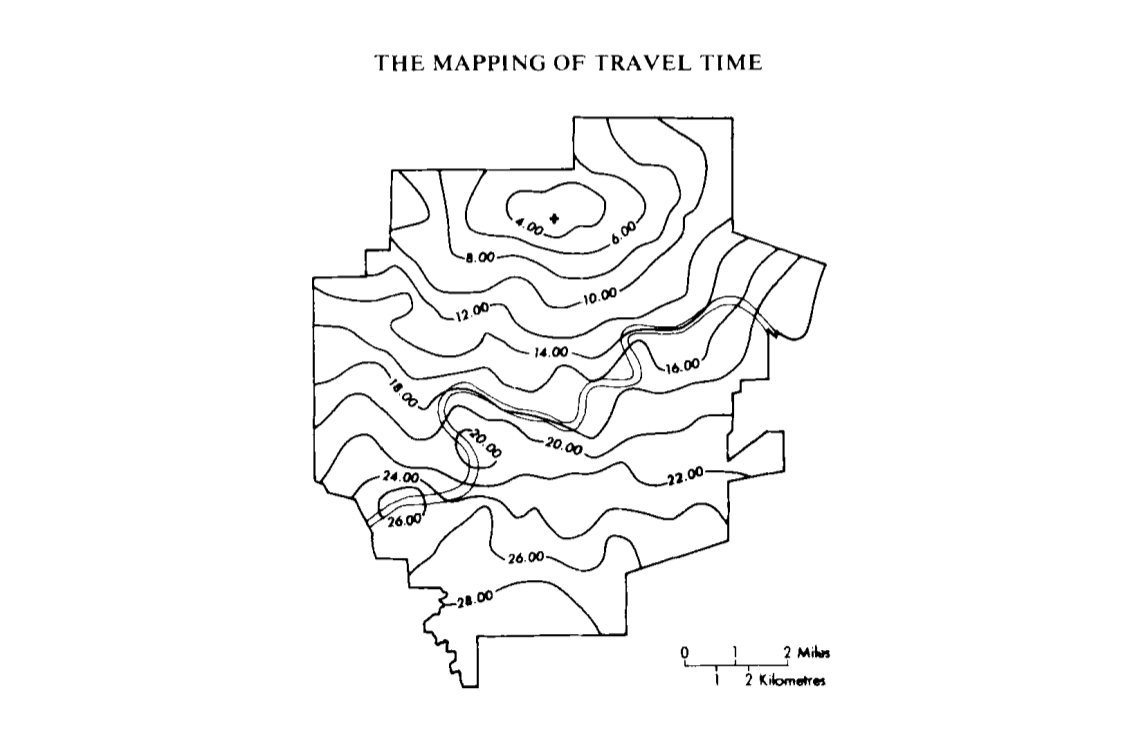
\includegraphics[width=0.32\textwidth]{./img/overv-maptt.png}}
      \label{fig:overv:1}
    \end{figure}

    In 1881, Francis Galton constructs the first isochronic map for the Royal
    Geographic Society (figure \ref{fig:overv:isopc}). It depicts the
    distances that can be traversed in equal times starting from London
    \cite{galton1881construction}. His contribution offers a polygonal
    generalization and suggests that future maps can be easily constructed for
    more detailed continental travel or home excursion maps.\par

    Among the first to define accessibility as indicator for urban
    transportation systems is Walter G. Hansen (1959). He presents a method for
    determining accessibility patterns within metropolitan areas and defines
    accessibility as the potential of opportunities for interaction serving
    residents in urban areas \cite{hansen1959accessibility}.\par

    % armstrong 1972
    % transport costs play an important role
    % here: economic evaluation of airports
    % road travel times and weighting by importance for the application and population
    %%% GRAPHIC FIG 3or4

    Pioneer in computing accessibility analysis on the foundation of
    transportation networks is Harvey W. Armstrong (1972) who converted an
    exemplary road network with 159 nodes to a matrix and used a C.D.C. 6000
    computer to evaluate economic feasibility of airports in South Hamphsire
    \cite{armstrong1972network} (figure \ref{fig:overv:nodac}).\par

    Jean-Claude Muller (1978) highlights issues with the mapping of
    time-distances as the derived space is often non-euclidean and hardly
    mappable without distorting the geographic reference system
    \cite{muller1978mapping}. He presents a numerical approach for time-distance
    transformations of Edmonton and analysis the resulting distortions (figure
    \ref{fig:overv:maptt}).\par

    \begin{figure}[ht]
      \subcaptionbox{
        \label{fig:overv:patnt}
        Method of Providing Travel Time, 2001
        \cite{ran2001method}.}
      {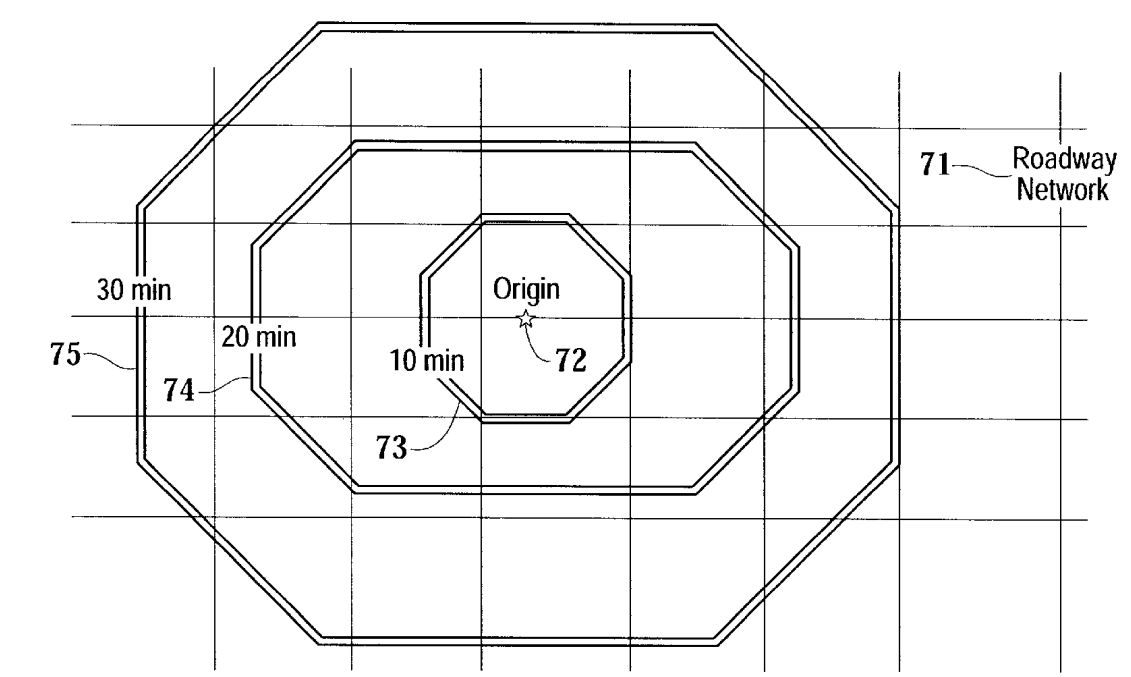
\includegraphics[width=0.32\textwidth]{./img/overv-patnt.png}}
      \hfill
      \subcaptionbox{
        \label{fig:overv:berln}
        Visualization of Quality of Mobility in Public Transport, 2010
        \cite{Glander2010}.}
      {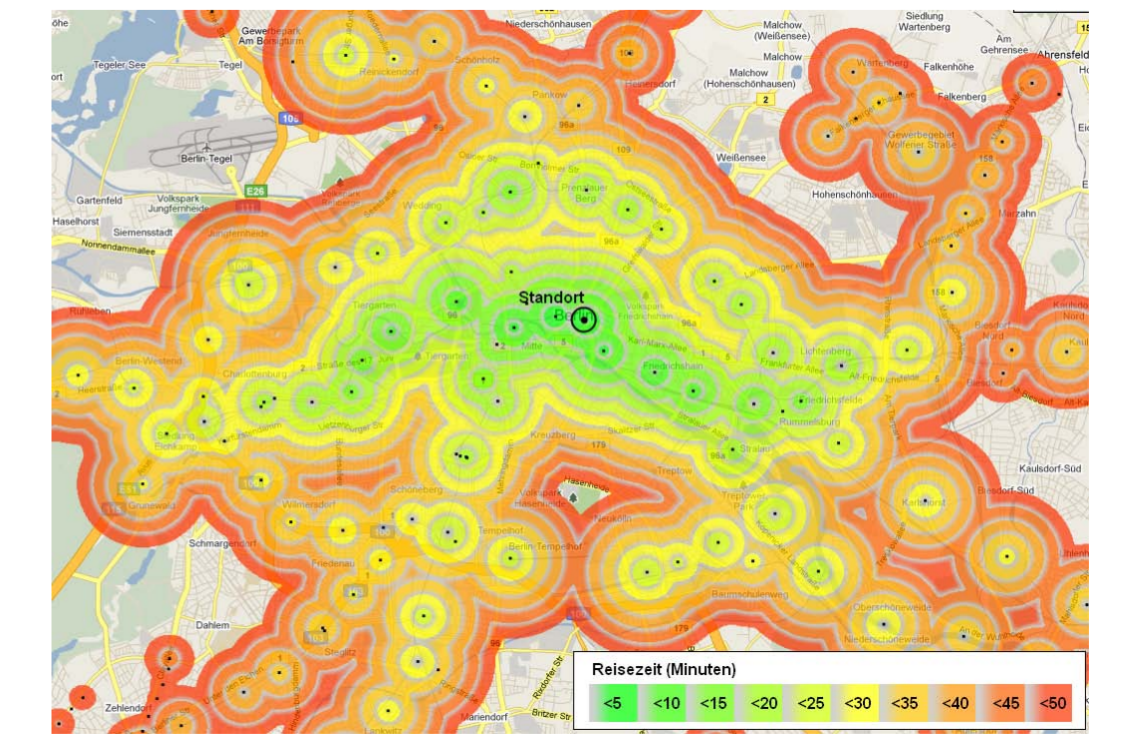
\includegraphics[width=0.32\textwidth]{./img/overv-berln.png}}
      \hfill
      \subcaptionbox{
        \label{fig:overv:potsd}
        Network-Based Accessibility Visualization in Potsdam, 2012
        \cite{hollburghier,Hollburg2014}.}
      {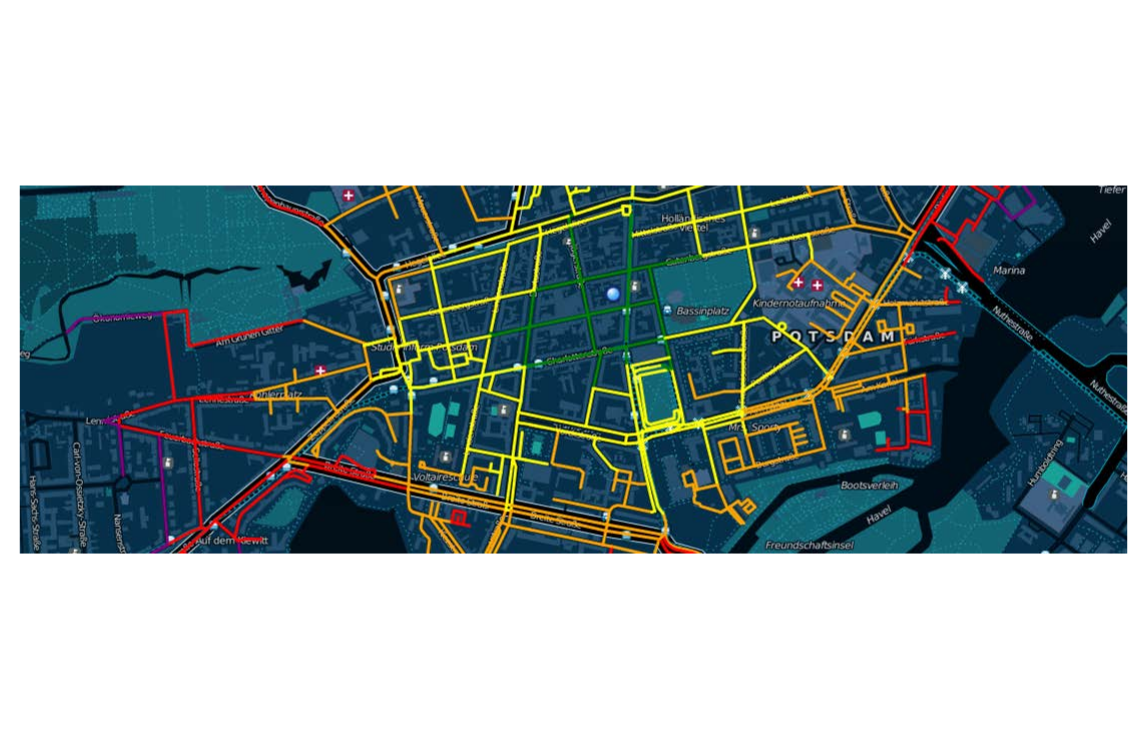
\includegraphics[width=0.32\textwidth]{./img/overv-potsd.png}}
      \caption{Shoo bar.}
      \label{fig:overv:2}
    \end{figure}

    The United States Patent and Trademark Office (\acrshort{uspto}) publishes
    the patent \#US006317686B1 issued by Bin Ran in 2001 on the method of
    providing travel time \cite{ran2001method}. It claims a personalized
    multi-modal travel prediction and trip decision support system including
    traffic forecast maps such as travel speed maps, travel time maps, and
    travel cost maps. It uses contour lines to represent predictive minimal
    travel time from a selected origin (figure \ref{fig:overv:patnt}).\par

    % street theis 2006
    % time based maps describe time accessibility of networks
    %%% FIG: 56 or 57 global integration of london (axial map) of network

    An important milestone and often cited reference is the final report on
    TimeContours by Nicholas Street (2006). It provides a Java application which
    maps isochrones onto public transport and road graphs to display
    transportation costs with respect to the travel time required
    \cite{street2006timecontours}. It discusses methods to display more than two
    dimensions on geographic maps such as isolines and defines isochrones --
    isolines of same time -- as derivation of the more commonly used isohypses
    -- isolines of the same height -- in a similar manner.\par

    % neis et al. 2007
    % utilizes attributed street network graph
    %%% FIG 13 accessibility maps buffer isolines convexhull

    A first web-based service for accessibility analysis is specified by
    Neis et al. (2007). Their approach suggests an accessibility analysis
    service (\acrshort{aas}) based on standards defined by the Open Geospatial
    Consortium (\acrshort{ogc}) \cite{neis2007webbasierte}. A provided web
    application is presented as Java Applet and receives responses in extensible
    markup language format (\acrshort{xml}). It calculates an elevation model
    where the third dimension encodes the required travel time and compares
    different visualization methods such as buffers, convex hulls and isochrones
    to display the results.\par

    A well organized summary on different methods for providing accessibility
    maps such as accessibility indices, anamorphosis maps or isochrone
    visualizations can be found in Martijn van Campenhout's thesis on travel
    time maps (2010) \cite{van2010travel}.\par

    % glander 2010
    % calculates isochrones from weighted voronoi centers (?) and distance fields
    %%% FIG 1 public transport berlin

    % müller 2010
    % distance transformations for accessibility mapping in public transport domain
    % for concurrent web based accessibility mapping
    % surface based (euclidean) vs network based (non euclidean) distance computation
    % first who highlights: display of network is no only effective for the user but efficient and correct calc'able
    % generalized polygons introduce visual errors and high rendering demand

    Glander et al. (2010) present an accessibility map visualization technique
    with a focus on polygon-based approaches in the public transport domain
    \cite{Glander2010} (figure \ref{fig:overv:berln}), and raster-based distance
    transforms~\cite{Mueller2010} which both lack precision in display offered
    by network-based approaches such as the one presented in this thesis.\par

    % innereber et al. isogar (2013)
    % figure (web app)

    % gortana 2014
    % isoscope web app
    % unified isochrone maps with time varying  travel data
    % instead multiple isolines for for travel times: mult isolines for times of day
    % reveals time-dependent spatial travel variance
    % FIG 1 24 layered shapes for each hour of the day

    % yin et al. 2015
    % integrated platform for accessibility analysis tasks
    % accessible to a wider range of audiences
    % FIG 4accessibility view (choropleth), travel time view (isochrone)

    The team around Yin et al. (2015) presents a web-based system for
    visualization of multi-modal accessibility for multiple land-uses. It
    highlights the importance of providing an easy-to-use web-interface as the
    users will not need to purchase or install software and therefore make the
    application accessible to a wider range of audiences~\cite{Yin2015}.
    However, the visualization technique does not focus on the specifics of
    transportation network representations.\par

    Finally, this thesis is furthering the work of Hollburg et al. (2012,
    2014) and the resulting services Motion Intelligence GmbH offers with their
    Route360°-\acrshort{js} \acrshort{api}. In \cite{hollburghier}, a web-based
    accessibility mapping service is provided to support tourists to assess
    reachability for points of interest (\acrshort{poi}) in the city of Potsdam.
    It provides a
    limited network-based visualization and highlights the benefits from
    mapping the travel times directly onto the transportation network rather
    than calculating isochrones (figure \ref{fig:overv:potsd}). However, it
    realizes it's not feasible to use this approach for larger networks
    including car travel or public transport. In \cite{Hollburg2014}, Hollburg
    presents an efficient way to generalize road segments and to calculate
    isochrones to visualize large accessibility maps in web clients and argues
    polygons are faster to transmit than complete network geometries due to the
    smaller data volume. The network-based method developed in his preceding
    work was comprehensible but not efficient for huge transportation networks.

  \section{Related applications and maps}
    \label{sec:overv:applc}

    % maps %%%%%%%%%%%%%%%%%%%%%%%%%%%%%%%%%%%%%%%%%%%%%%%%%%%%%%%%%%%%%%%%%%%%%

    % apps %%%%%%%%%%%%%%%%%%%%%%%%%%%%%%%%%%%%%%%%%%%%%%%%%%%%%%%%%%%%%%%%%%%%%

    Foo. Baz.

    % isoga, simplefleet, public transit travel time, simple online network analysis(hollburg 2014 FIG 7)
    % SONA (simple online network analysis)

%    Time Travel (Oskar Karlin) 2005
%
%http://www.oskarlin.com/2005/11/29/time-travel/
%
%Oskar Karlin. Time travel, 2005. URL http://www.oskarlin.com/2005/11/29/time-travel/.
%Letzter Zugriff: 31.1.2010.
%
%Time Travel, Oskar Karlin, http://www.oskarlin.com/2005/11/29/time-travel/
%[Accessed 04 Jan 2006]
%
%#######################
%http://www.openrouteservice.org/
%Accessibility Analysis
%
%#######################
%https://github.com/mapbox/osrm-isochrone
%
%#######################
%WalkScore Travel Time API
%https://www.walkscore.com/professional/travel-time-api.php
%
%#######################
%OneBayArea, San Fransisco Plan 2040
%http://maps.planbayarea.org/travel_housing/
%
%#######################
%Graphhopper Direction API
%Isochrone API
%https://graphhopper.com/api/1/docs/isochrone/
%
%#######################
%Hollburg et al (2014)
%https://www.route360.net/
%
%#######################
%http://cartoo.dyndns.org/


% https://www.khronos.org/news/press/significant-gltf-momentum-for-efficient-transmission-of-3d-scenes-models

% @TODO 2.3 ???

%!TEX root = ../schoedon.tex

%%%%%%%%%%%%%%%%%%%%%%%%%%%%%%%%%%%%%%%%%%%%%%%%%%%%%%%%%%%%%%%%%%%%%%%%%%%%%%%%
\cleardoublepage              %%% REQUIREMENTS                               %%%
\chapter{Requirements for this approach}
  \label{chap:requr}

  One way of communicating mobility information such as travel times are
  two-dimensional maps. Accessibility and mobility becomes a central topic in a
  growing number of fields. There are strong demands for corresponding web
  mapping components based on massive geo-data sets, such as \acrshort{osm}.\par

  An interactive visualization technique for web-based accessibility maps should
  adhere to the following requirements and challenges:\par

  \begin{enumerate}[\label=({R}1)]
    \item \label{enu:requr:r1} It should support a web-based,
      hardware-accelerated implementation using WebGL. %~\cite{Parisi2012}.
    \item \label{enu:requr:r2} It should utilize a standardized and compact
      data representation that allows for decoupling network geometry from
      temporal data to reduce data transmission and updates.
    \item \label{enu:requr:r3} It should enable interactive client-side
      filtering, mapping, and rendering for visual feedback.
    \item \label{enu:requr:r4} It should map the travel time information
      directly onto the transportation network for highly detailed
      visualizations.
  \end{enumerate}

  Requirement R\ref{enu:requr:r2}.

  \section{Web-based provision}
    \label{sec:requr:websd}
    This project focuses on the JavaScript webmapping framework \textit{Leaflet-JS} [??]. Better alternatives with a more advanced WebGL-integration are available (e.g. \textit{OpenLayers 3}) but a high compatibility with the existing \textit{Route360-JS} API developed by Motion Intelligence GmbH [??] is a requirement for this project. Therefore, Leaflet will be used.\par
    There is no native support for WebGL in Leaflet, yet\footnote{While writing this paper, a spanish software engineer, Iván Sánchez Ortega, started working on a Leaflet.GL plugin architecture [??] which was not taken into consideration as it is still experimental and was not available when this project implementation was started.}. Along with this implementation, a handful of Leaflet plugins will be developed which support a future WebGL integration [??][??] (see section {sec:tile}).\par
    % compare expert knowledge w/ GIS systems

  \section{Compact data representation}
    \label{sec:requr:data}

  \section{Client-side mapping and rendering}
    \label{sec:requr:clien}
    % user foo interaction, dynamic bar

  \section{Network-based visualization}
    \label{sec:requr:netwr}

%%%%%%%%%%%%%%%%%%%%%%%%%%%%%%%%%%%%%%%%%%%%%%%%%%%%%%%%%%%%%%%%%%%%%%%%%%%%%%%%

%!TEX root = schoedon.tex

%%%%%%%%%%%%%%%%%%%%%%%%%%%%%%%%%%%%%%%%%%%%%%%%%%%%%%%%%%%%%%%%%%%%%%%%%%%%%%%%
\cleardoublepage              %%% CONCEPT                                    %%%
\chapter{Conception of glTF Tiling}
  This section briefly discusses design decisions on web-mapping frameworks, data
  formats, and required geographic projections. To evaluate the concepts based on
  real-world data sets, we choose to rely on the Route360-JS$^\circ$ API for server-side
  computing of routing data. Although there are alternatives with advanced WebGL-integrations
  available (e.g., OpenLayers 3, Cesium), this work focuses on the web-mapping framework
  Leaflet-JS for interoperability with the Route360$^\circ$-JS API. However, the
  glTF-based approach is not specific to Leaflet and can be integrated into other
  web-mapping frameworks.\par
  The exemplary transportation network used in this paper is a part of an OSM data
  set of Berlin. It comprises streets, footways, and data of the transportation
  infrastructure network. Based on this network a single-source shortest-path accessibility
  analysis \cite{Meyer2001} is performed using the Route360$^\circ$-JS API. It results in
  the travel times required by foot, bicycle, car, or public transportation from a
  single starting point to all remaining nodes of the network. The geometry, topology,
  and accessibility data (represented on a per-node basis) is stored in a database which
  is used for data conversion to the file formats of our visualization techniques.\par

  \section{Preliminaries and assumptions}
    \subsection{Open geographic data sets}
    \subsection{Geographic projections}
      To minimize the processing of data and allow easy GL-transformations, it's important to reduce reprojections and avoid spherical units (e.g. degree, lat/lon).\par
      Leaflet uses the \texttt{EPSG:4326} standard projection which is the world geodetic system 1984 (WGS84) and uses a latitude/longitude coordinate format. This means, all programming interfaces of Leaflet return values in degree.\par
      Internally, Leaflet uses \texttt{EPSG:3857}, the web mercator projection, a metric system going back to Gerard Mercator's flat world map in 1569 [25]. It uses northing and easting as a measure of distance in meters from the equator and the prime meridian. This is already an advantage over WGS84 as it does not require computing-intense spheric transformations in calculations. Unfortunately, Leaflet does not allow access to the internal metric system without automatically triggering one or more reprojections from/to WGS84 [23].\par

%%%      \begin{figure}[h]
%%%        \centering
%%%        \includegraphics[width=0.3\textwidth]{resources/earth-256.pdf}
%%%        \caption{The world in 256 square pixels.}
%%%        \label{fig:earth256}
%%%      \end{figure}

      To simplify the geographic coordinates, all geographic references will be projected on a single tile of size 256*256 pixel with it's origin in the north-west corner (see figure \ref{fig:earth256}). In this reference system, the Brandenburg Gate in Berlin would be at pixel coordinate \texttt{[137.51253, 83.9612]}. This allows enough precision, moves as close as we can get to hardware-coordinates and is still device-independent.\par

      To minimize the client-side data processing and to reduce transformation operations,
      it's important to reduce re-projections and avoid spherical units (e.g., degree,
      latitude/longitude). Leaflet-JS uses the EPSG:4326 standard projection, which is
      the world geodetic system 1984 (WGS84) and uses a latitude/longitude coordinate
      format, thus all programming interfaces of Leaflet return values in degree.
      To remove the need for computing-intense spherical transformation and to simplify
      coordinates, all geographic references are projected to a normalized range $[0, 1]$
      with it's origin in the north-west corner. This moves as close as we can get to
      hardware-coordinates and conveys device-independence.\par
      To dis\-play geographic coordinates in Mercator projection (EPSG:3857) on a GPU-rendered
      map, two major steps have to be performed. First, the geographic projection of
      each coordinate has to be transformed into a normalized projection by translating
      the coordinate origin to the top-left corner by the distance of half an equator.
      Further, the units will be scaled from 40.075.016 meters to a normalized range
      of~$[0,1]$. Finally, this projection has to be transformed to screen space coordinates
      of the current device viewport.  The device coordinate origin will be translated
      to the top-left corner of the visible viewport. The geometry view will be scaled
      using the current zoom level scale factor and visible canvas size. The top-left
      corner of the map can be retrieved from Leaflet-JS and used as an offset for
      the model view to translate to the displayed geometries~(Fig.~\ref{WD:Fig:ViewportMapping}).
    \subsection{Transportation modes}
    \subsection{Backend specification}
    \label{sec:conc:back}
      %%%\pfinal
      %%%\highinlinetodo{Integrate back-end specification.}
      %%%\pprelim
      %preprocessing of the network geometry
      %goal reduce computations required for browser based mapping and rendering
      %given geographic network coordinates (lat,lon)
      %required coordinate representation close to rendering
      %approach compute webgl optimized tiles in normalized reference system
      % encode tiles using a specific transmission format
      % network preprocessing is only required once
    \subsection{Transmission formats}
      Due to the data-intense applications in webmapping services, most implementations follow a client/server model. It's important to research and evaluate options on exchange formats for the underlying geodata.\par
      The following formats are considered worth for comparison.
      \begin{itemize}
      \item In computer graphics, the COLLADA digital asset exchange format (\texttt{.dae}) is used for modelling purposes and exchange of editable 3D models.
      \item The new OpenGL transfer fromat (\texttt{.gltf}) is currently being drafted by the Khronos Group [13] and promises to be a file format more close to the hardware requirements.
      \item In geoinformation sciences, GeoJSON is a JavaScript object notation (\texttt{.json}) which is extended by geographic features with geometries and properties.
      \item The Geography Markup Language (\texttt{.gml}) is an XML grammar for expressing geographical features.
      \end{itemize}
      Formats not taken into account are KML, Google's equivalent to GML, and TopoJSON, another JSON format with merged geometry fields. In addition, raster data formats are ignored as they do not store any extractable geometry information.\par
      Table \ref{tab:dataform} compares the stated formats and evaluates both, their space-complexity and postprocessing requirements. The space-complexity is important to evaluate the required bandwidth for the application. The postprocessing is the aforementioned bottleneck in performance of transforming geographic data into close-to-hardware array buffers for the GPUs.\par

%%%      \begin{table}[!h]
%%%        \centering
%%%        \begin{tabular}{l|c|l}
%%%          Format & Space-Complexity & Client-Postprocessing\\ \hline
%%%          \cellcolor{yellow!15}.dae.gz & \cellcolor{green!15}\texttt{++} & \cellcolor{red!15}required, decompress \\
%%%          \cellcolor{green!15}.bgltf & \cellcolor{green!15}\texttt{+o} & \cellcolor{green!15}not required \\
%%%          \cellcolor{yellow!15}.gltf.gz & \cellcolor{green!15}\texttt{+o} & \cellcolor{yellow!15}decompress only \\
%%%          \cellcolor{yellow!15}.dae & \cellcolor{yellow!15}\texttt{oo} & \cellcolor{red!15}required \\
%%%          \cellcolor{yellow!15}.gltf & \cellcolor{red!15}\texttt{o-} & \cellcolor{green!15}not required \\
%%%          \cellcolor{red!15}.json & \cellcolor{red!15}\texttt{o-} & \cellcolor{red!15}required \\
%%%          \cellcolor{red!15}.gml & \cellcolor{red!15}\texttt{---} & \cellcolor{red!15}required \\
%%%        \end{tabular}
%%%        \caption{Comparison of data formats}
%%%        \label{tab:dataform}
%%%      \end{table}
      Concerning the space requirements, both glTF and COLLADA perform above average. Base of the comparison are the Cesium Milk Truck and Cesium Man by Analytical Graphics Inc [9]. The binary version of glTF (\texttt{.bgltf}) is even smaller than a gzipped version (\texttt{.gltf.gz}). Classic geodata formats fail in terms of space-complexity since both, JSON and XML formats are quite bloated.\par
      Concerning the client-side postprocessing requirements, only the OpenGL transfer format allows to store array buffers which eleminates any javascript processing other than requesting and reading the data. This is an obvious knockout criteria for the other candidates and therefore glTF will be considered the best choice for this application. Details on the postprocessing issues will be discussed in section \ref{sec:issue}.\par
      For handling data-intense client/server communication, it is important to
      evaluate options on data exchange formats. Both, Coughlin and Trevett motivate
      why a standardized data format close to hardware devices for applications on the
      web are required \cite{Coughlin2014,Trevett2012}. We considered the following file
      formats for comparison: (1) COLLADA this digital
      asset exchange format (\texttt{.dae}) has been established for modeling purposes
      and exchange of geometry and scene descriptions~\cite{Barnes2008}; (2) the Geography
      Markup Language (\texttt{.gml}) is based on a~XML grammar standardized by the Open
      Geospatial Consortium~(OGC) to represent geographical features~\cite{GML2007}; (3)
      GeoJSON (\texttt{.json}) a JavaScript object notation that is extended by geographic
      features comprising geometries and its properties~\cite{Butler2008}; and (4) the
      OpenGL transmission format (\texttt{.gltf}) was recently released by Khronos Group
      and is designed to be a file format close to the requirements of the rendering
      hardware~\cite{Cozzi2015}. Table~\ref{WD:Tab:DataFormats} (next page) compares
      the file formats with respect to their memory footprint and client-side processing
      requirements. The former is important to evaluate the required bandwidth, while
      the processing is the aforementioned bottleneck in performance of transforming
      geographic data into GPU array-buffers.

      %%%%%%%%%%%%%%%%%%%%%%%%%%%%%%%%%%%%%%%%%%%%%%%%%%%%%%%%%%%%%%%%%%%%%%%%%%%%%%%
      %%
      %% Table: Data Formats
      %%
      %%%%%%%%%%%%%%%%%%%%%%%%%%%%%%%%%%%%%%%%%%%%%%%%%%%%%%%%%%%%%%%%%%%%%%%%%%%%%%%
%%      \begin{table}[tb]
%%      \centering
%%      \begin{tabular}{|l|r|l|}
%%       \hline
%%        \textbf{Format}                     & \textbf{Memory (Byte)}    & \textbf{Client Processing}\\\hline
%%        \cellcolor{red}\texttt{.dae.gz}     & \cellcolor{green}54,949   & \cellcolor{red}required, decompress \\
%%        \cellcolor{yellow}\texttt{.gltf.gz} & \cellcolor{green}58,791   & \cellcolor{yellow}decompress only \\
%%        \cellcolor{red}\texttt{.json.gz}    & \cellcolor{green}67,693    & \cellcolor{red}required, decompress \\
%%        \cellcolor{green}\texttt{.glb}      & \cellcolor{green}89,168   & \cellcolor{green}not required \\
%%        %\cellcolor{green}\texttt{.bgltf}    & \cellcolor{green}89,514   & \cellcolor{green}not required \\
%%        \cellcolor{yellow}\texttt{.gltf}    & \cellcolor{yellow}173,597 & \cellcolor{green}not required \\
%%        \cellcolor{red}\texttt{.gml.gz}     & \cellcolor{yellow}211,137 & \cellcolor{red}required, decompress\\
%%        \cellcolor{red}\texttt{.dae}        & \cellcolor{yellow}212,788 & \cellcolor{red}required \\
%%        \cellcolor{red}\texttt{.json}       & \cellcolor{red}824,790    & \cellcolor{red}required \\
%%        \cellcolor{red}\texttt{.gml}        & \cellcolor{red}2,698,953   & \cellcolor{red}required \\
%%        \hline
%%      \end{tabular}
%%      \caption{Comparison and rating (dark background means not suitable) of data formats
%%      with respect to the amount of memory required for server-to-client data  transmission
%%      and client-side processing prior to rendering. The data set used for comparison
%%      comprises 1840 vertices and 3624 faces (no texture data included).}
%%      \label{WD:Tab:DataFormats}
%%      \afterFloat
%%      \end{table}
      %%%%%%%%%%%%%%%%%%%%%%%%%%%%%%%%%%%%%%%%%%%%%%%%%%%%%%%%%%%%%%%%%%%%%%%%%%%%%%%

      Concerning memory consumptions, both glTF and COLLADA perform above average. The
      comparison uses the Cesium Milk Truck (provided by Analytical Graphics Inc.). As
      a result, the gzipped version of glTF (\texttt{.gltf.gz}) is more compact than a
      binary version (\texttt{.glb}). Due to high memory footprints, traditional
      geodata formats (esp. JSON and GML) are not suitable for our approach (cf. R2). Further,
      regarding the client-side processing requirements prior to rendering, the OpenGL
      transfer format allows to store array buffers which eliminates any JavaScript
      processing except requesting and reading the data. Due to this, and by respecting~
      R1~and~R3, the glTF file format is considered to be the best choice.

      % table all formats
      % conclude gltf is awesome
  \section{Mapping and rendering logic}
    To display geographic coordinates on a GPU-rendered map, two major steps have to be performed.\par
    First, the geographic projection has to be transformed into a pixel projection. Therefore, the coordinate origin has to be moved to the topleft corner by translating it along the x-axis and the negative y-axis for half an equator. The units will be scaled from 40.075.016 meters to 256 pixels.

%%%    \begin{figure}[h]
%%%      \centering
%%%      \includegraphics[width=0.3\textwidth]{resources/viewport.pdf}
%%%      \caption{Viewport coordinates overview.}
%%%      \label{fig:viewport}
%%%    \end{figure}

    Finally, this pixel projection has to be made visible in the current viewport of the client's device. The device coordinate origin will be translated to the topleft corner of the visible viewport. The model view will be scaled using the current zoom level scale factor and visible canvas size.  The topleft corner of the map can be retrieved from Leaflet and used as an offset for the model view to translate to the displayed geometries (figure \ref{fig:viewport}).\par
    % reduced mapping overhead due to
    % tiled network geometry is decoded to rendering representation
    % no coordinate transformations required
    % corresponding travel times stored in separate vertex buffer object
    % webgl based gpu rendering as map overlay
    % direct buffer upload to gpu
    % color gradient textures used by fragment shader
%%%%%%%%%%%%%%%%%%%%%%%%%%%%%%%%%%%%%%%%%%%%%%%%%%%%%%%%%%%%%%%%%%%%%%%%%%%%%%%%

%!TEX root = ../schoedon.tex

%%%%%%%%%%%%%%%%%%%%%%%%%%%%%%%%%%%%%%%%%%%%%%%%%%%%%%%%%%%%%%%%%%%%%%%%%%%%%%%%
\cleardoublepage              %%% IMPLEMENTATION                             %%%
\chapter{Web-based proof-of-concept}
  \label{chap:imple}
  A proof-of-concept implementation is provided along with this thesis. This
  chapter covers the Leaflet-JS integration details. It is targeted to work with
  web applications and mobile devices. In the following subsections the
  challenges with the web-based provision are examined. The architecture will be
  explained and the resulting applications will be presented.\par

  \section{Architecture overview}
    \label{sec:imple:archi}
    The implementation requires a client/server architecture which offers both,
    a tiling service supplying the pre-calculated glTF tiles and a routing
    service supplying travel times on-request at runtime (figure
    \ref{fig:imple:archi}).\par

    \begin{figure}[h]
      \centering
      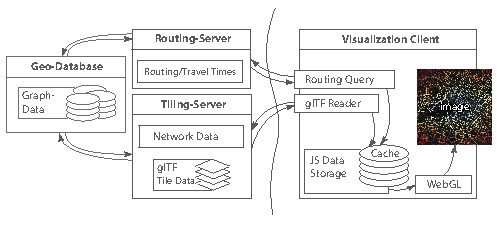
\includegraphics[width=\linewidth]{./img/conceptual-overview-bw.pdf}
      \caption{Architecture of preprocessing back-end and visualization client.}
      \label{fig:imple:archi}
    \end{figure}

    The back-end consists of three components:\par

    \begin{description}
      \item[Geo-Database] A geographic database server contains the street and
        transportation networks. It maintains updates from a remote geo-data
        source, e.g., OpenStreetMap, and processes the data into a
        routing-enabled graph representation.
      \item[Tiling-Server] A tiling server processes the static network data
        into a tiled glTF data set. This data only has to be generated once and
        will be available on-demand for any future geometry requests.
      \item[Routing-Server] A routing server handles dynamic requests based on
        the user's selected starting location, transportation type and maximum
        travel time. It responds with customized routing information for the
        underlying transportation network.
    \end{description}

    The front-end contains the mapping and rendering stages. A glTF reader will
    request and load the network geometries. Based on the user inputs, routing
    data will be queried. All responses are mapped, cached and rendered in the
    client.\par

    As described in section \ref{sec:conct:preli:backe}, the back-end is not
    subject to further technical specification in this document. Therefore, the
    following applications strongly focus on the front-end implementation and
    visualization.\par

  \section{Iterative development process}
    \label{sec:imple:cycle}
    The implementation is solved by an evolutionary prototyping process.\par

    To allow a fast evaluation of the results gained during the different stages
    of development, an evolutionary development process is used. It leads to
    multiple proof-of-concept versions which can be analyzed afterwards.\par

    A working back-end -- as specified in section \ref{sec:conct:preli:backe} --
    provides the prototypes with real-time data at run-time. It is provided and
    maintained by Motion Intelligence GmbH. By utilizing and extending the
    existing Route360-JS API [??], compatibility and potential future
    integrations are maintained.\par

  \section{Proof-of-concept applications}
    \label{sec:imple:applc}
    In the following sections, three major proof-of-concept implementations will
    be presented:\par

    \begin{description}
      \item[PoC\#1 Leaflet-JS with CPU native lines vector
        tiling] This implementation is not interesting for
        this work as it neither uses WebGL nor glTF and is only implemented to
        have a classic approach available. In addition, the performance of the
        first prototype is very low, even for small accessibility map
        visualizations (below 10 minutes travel time complexity in a city
        center, compare section \ref{sec:imple:applc:nativ}).
      \item[PoC\#2 Leaflet-JS with GPU-enabled canvas overlay and vector tiling]
        This prototype is interesting both for the successful
        WebGL integration in Leaflet-JS and the issues arising with GeoJSON
        post-processing. See section \ref{sec:imple:applc:vectr} for more
        details.
      \item[PoC\#3 Leaflet-JS with GPU buffer tiling] This approach
        is implementing a GPU buffer tiling service explicitly utilizing the
        glTF data exchange format. See section \ref{sec:imple:applc:tgltf} for
        more details.
    \end{description}

    \subsection{Leaflet-JS native network rendering}
      \label{sec:imple:applc:nativ}
      A reference implementation in Leaflet-JS is provided (figure
      \ref{fig:imple:applc:nativ}). It does not utilize hardware acceleration or
      WebGL rendering. It processes the vector data in GeoJSON format using the
      native Leaflet-JS JavaScript class \texttt{L.GeoJson}. Therefore, both the
      mapping and rendering will be performed on CPU.\par

      \begin{figure}[h]
        \centering
        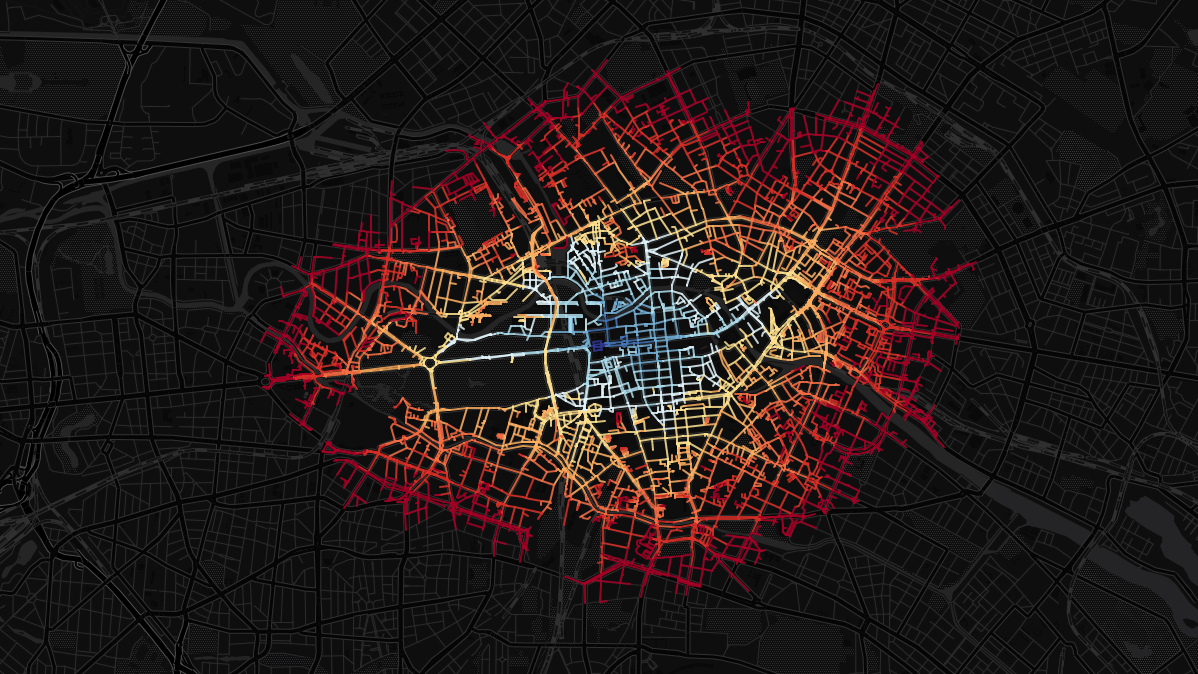
\includegraphics
          [width=0.7\linewidth]
          {./img/screenshot-poc1-600s-native.png}
        \caption{An accessibility map rendered native with Leaflet-JS vector
          tiles in GeoJSON format. The selected transportation mode is walking
          and the displayed travel time is 10 minutes.}
        \label{fig:imple:applc:nativ}
      \end{figure}

      The rendered street network for 600 seconds travel time in walking mode
      contains 13,829 features (25,821 vertices). It shows a major performance
      bottleneck for both the mapping and the rendering stage. It wont be
      evaluated any further and is only used for the performance comparison in
      section \ref{sec:evalu:pcomp} as native Leaflet-JS reference without
      WebGL hardware acceleration.\par

    \subsection{WebGL with tiled vector data}
      \label{sec:imple:applc:vectr}
      Leaflet-JS provides a 2D \texttt{L.map()} canvas on a
      \texttt{<div id="map" />} HTML DOM element. This can be used for basic web
      mapping tools like raster base tiles or simple vector items. The extended
      class \texttt{L.canvasOverlay()} by Sumbrera (2015) [??] provides
      Leaflet-JS with a 3D overlay which handles redrawing of the canvas and
      therefore allows basic WebGL context integration (figure
      \ref{fig:imple:applc:overlay}).\par

      % https://blog.sumbera.com/2014/04/20/leaflet-canvas/

      \begin{figure}[h]
        \centering
        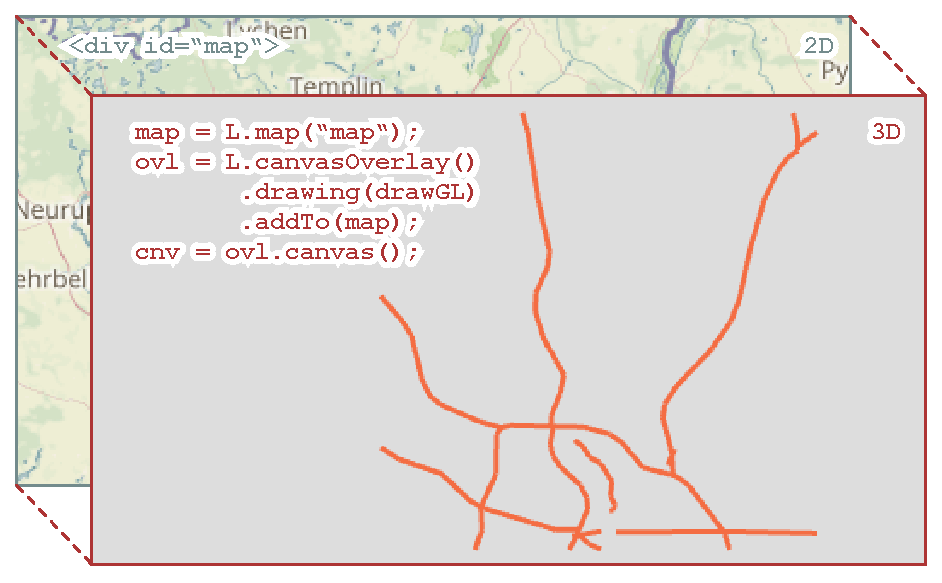
\includegraphics[width=0.7\linewidth]{./img/leaflet-canvas-overlay.pdf}
        \caption{Leaflet-JS canvas overlay schematic: A 2D map canvas is provided by Leaflet, the overlay class allows the rendering of 3D contexts.}
        \label{fig:imple:applc:overlay}
      \end{figure}

      On each map interaction, a \texttt{drawGL()} rendering call will be
      triggered by the overlay. This function reads the underlying GeoJSON and
      extracts all geographic features. For each feature in the feature-set, the
      algorithm checks the travel time properties and decides whether the
      feature is visible (below selected threshold) or not.\par

      Each visible feature will be converted to typed array buffers for vertices
      and colours. Each coordinate of the geometry has to be mapped to pixel
      coordinates (see section \ref{sec:conct:preli:gproj}).\par

      %%% @TODO below %%%

      The Leaflet-JS web-mapping framework does not offer any WebGL support, yet. Sumbrera [??] published a Leaflet-JS canvas overlay class which provides a generic overlay over the map canvas and handles view-port coordinates and drawing events.\par
      \lstinputlisting[float,caption={Leaflet-JS canvas overlay},label={lst:poc:overlay}]{./lst/leaflet-canvas-overlay.js}
      While Leaflet-JS provides a map canvas on a HTML DOM element (e.g., \texttt{<div id='map'>}) for two dimensional vector and raster contexts, Figure {fig:poc:overlay} shows how the \texttt{L.CanvasOverlay} class provides an additional context. The overlay can be used for custom HTML5 elements and handles view port coordinate alignment along with the underlying map. Furthermore, it can be utilized to bind a three dimensional context like WebGL and to handle the redrawing of the scene each time the map view changes (Listing {lst:poc:overlay}).\par
      \begin{figure}[h]
        \centering
        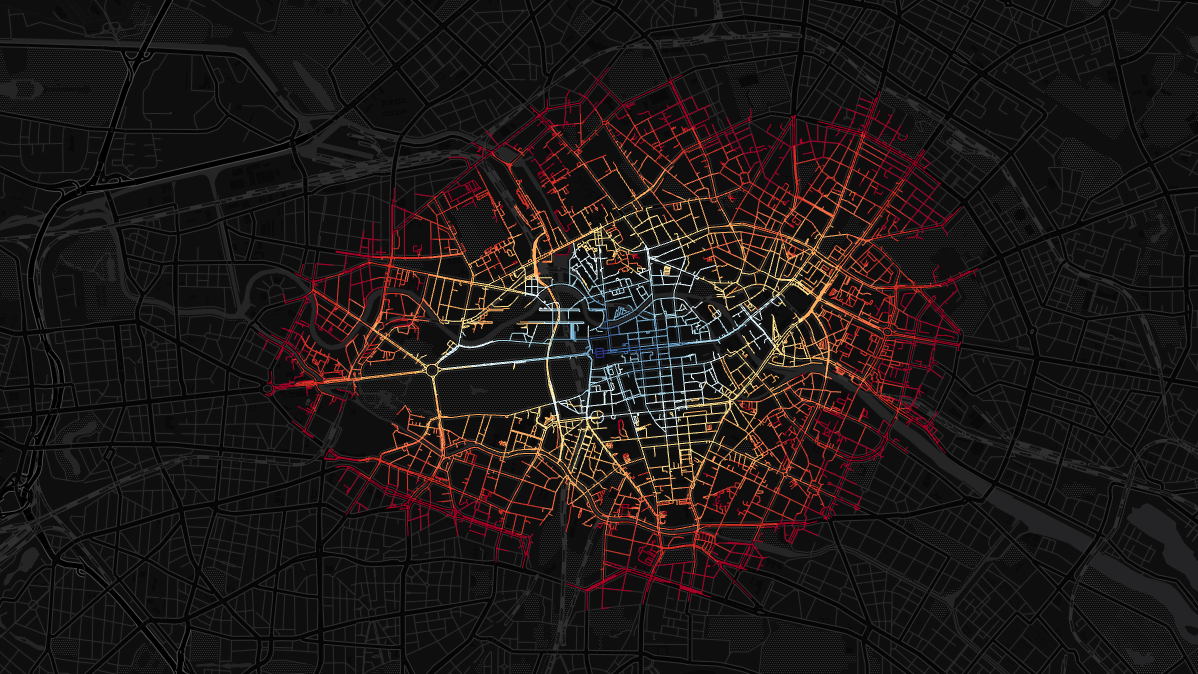
\includegraphics[width=0.7\linewidth]{./img/screenshot-poc2-600s-vector.png}
        \caption{An accessibility map rendered with WebGL on a Leaflet-JS canvas overlay utilizing vector tiles in GeoJSON format. The selected transportation mode is walking and the displayed travel time is 10 minutes.}
        \label{fig:poc:two}
      \end{figure}
      This implementation shows two issues.\par
      A blocking performance issue is the conversion from geodata to array buffers. For the mentioned dataset of only 15 minutes travel time this results in an iteration over 29.864 geographic features. In addition, the coordinates have to be iterated as well, leaving this example with 129.034 spheric conversions for 64.517 coordinates.\par
      Another problem is the unability to access the internal \texttt{EPSG :3857} metric coordinates from Leaflet. All positions have to be transformed using compute-intense spherical (degree) rather than optimized metric conversions [??].\par
      Leaflet-JS provides a 2D canvas on a HTML DOM element that is used for basic
      web-mapping tools such as raster-based tiles or simple vector items. An extended
      \textsl{canvas overlay} class provides Leaflet-JS with a 3D overlay that handles
      re-drawing of the canvas and enables basic WebGL context integration. On each map
      interaction, a draw call is issued by the overlay. This function processes the
      underlying GeoJSON and (1) extracts all geographic features, (2) marks each feature
      visible, if its travel time is below a user-selected threshold, and (3) converts
      each visible feature to typed array buffers (vertices and colors), including coordinate mapping.\par
      This implementation approach shows two performance bottlenecks: (1) the conversion
      from geodata representation to GPU array-buffers and (2) coordinate transformations
      for rendering~(cf.~Sec.~{WD:SubSec:PerformanceEvaluation}). \par
    \subsection{WebGL with tiled glTF data}
      \label{sec:imple:applc:tgltf}
      Table {tab:tilopts} highlights the advantages of geometry tiling. The layout stays dynamic and can be adjusted at runtime by custom user inputs similar to vector tiling approaches.\par
      The data processing is moved from client-side to server-side similar to raster tiling approaches. The result is high runtime preformance with low latencies and the resulting geometries can be cached client-side.\par
      The rendering happens on dedicated graphic devices and ensures outstanding performance even for complex geodata sets.

%%%      \begin{table}[!h]
%%%        \centering
%%%        \begin{tabular}{l|l|l|l}
%%%          Tile & Layout & Processing & Rendering\\ \hline
%%%          \cellcolor{yellow!15}Raster & \cellcolor{red!15}static & \cellcolor{green!15}Server & \cellcolor{red!15}Server\\
%%%          \cellcolor{yellow!15}Vector & \cellcolor{green!15}dynamic & \cellcolor{red!15}Client/CPU & \cellcolor{green!15}Client/GPU\\
%%%          \cellcolor{green!15}Geometry & \cellcolor{green!15}dynamic & \cellcolor{green!15}Server & \cellcolor{green!15}Client/GPU\\
%%%        \end{tabular}
%%%        \caption{Tiling options}
%%%        \label{tab:tilopts}
%%%      \end{table}
      Figure {fig:geotile} shows a screenshot of a modified version of the 4th prototype. It displays the geometry tile \texttt{[2200,1343]} at zoom level 12 rendered with WebGL using random colours.

%%%      \begin{figure}[h]
%%%        \centering
%%%        \includegraphics[width=0.475\textwidth]{resources/geometry-tile.png}
%%%        \caption{Geometry tile rendered with WebGL.}
%%%        \label{fig:geotile}
%%%      \end{figure}
      Two Leaflet-JS plugins are being developed to manage the tiling data logic [??].\par
      \begin{itemize}
        \item \texttt{L.TileBuffer} is the actual class for all geometry tiles. Each instance has the properties of \texttt{x}, \texttt{y} and \texttt{zoom}. In addition it stores the three required typed array buffers to render the tile with WebGL: a \texttt{Float32Array} for vertices, a \texttt{Uint16Array} for indices and a \texttt{Float32Array} for colours. This information is enough to render the complete tile in a single draw call.
        \item \texttt{L.TileBufferCollection} is a class which implements the basic tile caching logic. It has a \texttt{zoom} and a \texttt{size} property. In addition, it holds a collection of \texttt{L.Tile\-Buffer} objects for the current zoom level. As soon as the client requests a redraw of the scene, the collection can be rendered based on zoom and position of the visible tiles.
      \end{itemize}
      On each load event of a tile, Leaflet-JS will request the geometry (vertices and indices) from the tiling server and the travel times (colours) from the routing server. These three arrays are recieved in glTF format. They are used to create \texttt{L.TileBuffer} objects (figure {fig:tbuff}).\par

%%      \begin{figure}[h]
%%        \centering
%%        \includegraphics[width=0.3\textwidth]{resources/classes.pdf}
%%        \caption{Two Leaflet-JS plugins for geometry tiling.}
%%        \label{fig:tbuff}
%%      \end{figure}

      This approach eliminates client-side data processing and represents a new geometry-tiling
      approach based on glTF and following the common approach to partition map data
      into portions of similar size. Figure~{WD:Fig:ConceptualOverview} shows an conceptual
      overview of our approach: (1) the input transportation network will be pre-processed
      to glTF-tiles that are stored on a dedicated tiling server. In this step all
      coordinate transformations required for rendering are performed and a correspondence
      to the routing graph is established; (2) the visualization client queries the
      geometry of the tiles according to the current viewport and request travel times
      respectively by using the graph correspondence; (3) for visualization, the network
      tiles are cached and directly used for mapping and rendering.\par
      Table~{WD:Tab:TilingOptions} highlights the advantages of glTF-tiling. It
      supports client-side mapping (e.g., color mapping and lines styles) at runtime
      on according to user inputs without retransmission of data, similar to vector
      tiles. The data processing is transferred from client to server-side, similar
      to raster-tiling approaches. This results in high run-time performance with
      low latencies and the resulting geometries can be cached client-side. The
      rendering is performed on dedicated GPU using WebGL and thus ensures real-time
      performance for geometrical complex geodata sets.\par

      %%%%%%%%%%%%%%%%%%%%%%%%%%%%%%%%%%%%%%%%%%%%%%%%%%%%%%%%%%%%%%%%%%%%%%%%%%%%%%%
      %%
      %% Table: Tiling approaches
      %%
      %%%%%%%%%%%%%%%%%%%%%%%%%%%%%%%%%%%%%%%%%%%%%%%%%%%%%%%%%%%%%%%%%%%%%%%%%%%%%%%
%%      \begin{table}[b]
%%      \centering
%%      \beforeTable
%%      \begin{tabular}{|c|c|c|c|}
%%        \hline
%%        \textbf{Tiling Approach}  & \textbf{Processing}       & \textbf{Mapping}         & \textbf{Rendering}\\ \hline
%%        \cellcolor{yellow}Raster  & \cellcolor{green}Server   & \cellcolor{red}static    & \cellcolor{red}Server\\
%%        \cellcolor{yellow}Vector  & \cellcolor{red}Client/CPU & \cellcolor{green}dynamic & \cellcolor{green}Client/GPU\\
%%        \cellcolor{green}glTF     & \cellcolor{green}Server   & \cellcolor{green}dynamic & \cellcolor{green}Client/GPU\\
%%        \hline
%%      \end{tabular}
%%      \caption{Comparison and rating (dark background means not suitable) of tiling
%%      approaches with respect to the requirements of data processing, mapping, and
%%      rendering.}
%%      \label{WD:Tab:TilingOptions}
%%      \afterFloat
%%      \end{table}
      %%%%%%%%%%%%%%%%%%%%%%%%%%%%%%%%%%%%%%%%%%%%%%%%%%%%%%%%%%%%%%%%%%%%%%%%%%%%%%%

%%%%%%%%%%%%%%%%%%%%%%%%%%%%%%%%%%%%%%%%%%%%%%%%%%%%%%%%%%%%%%%%%%%%%%%%%%%%%%%%

%!TEX root = ../schoedon.tex

%%%%%%%%%%%%%%%%%%%%%%%%%%%%%%%%%%%%%%%%%%%%%%%%%%%%%%%%%%%%%%%%%%%%%%%%%%%%%%%%
\cleardoublepage              %%% EVALUATION                                 %%%
\chapter{Application examples and performance evaluation}
  \label{chap:evalu}
  \section{Applications in cooperation with Motion Intelligence GmbH}
    \label{sec:evalu:applc}

    % Planning, Real Estate, Tourism and Leisure, Market Research, Media

    \subsection{Business location finder}
      \label{sec:evalu:applc:busin}
    \subsection{Property market analysis}
      \label{sec:evalu:applc:propt}
    \subsection{Spare-time activity planning}
      \label{sec:evalu:applc:spare}
  \section{Comparison of the presented approaches}
    \label{sec:evalu:pcomp}
%%        \begin{figure*}[!htb]
%%    \centering
%%    \subfigure[Mapping]{
%%    \begin{tikzpicture}[font=\footnotesize] % mapping
%%    \begin{axis}[
%%    height=0.28\textwidth,
%%    width=0.5\textwidth,
%%    xmin=1,
%%    xmax=11,
%%    %xlabel={Selected Traveltime [min]},
%%    ymin=0.1,
%%    ymax=10000,
%%    %ylabel={Data Mapping Time [ms]},
%%    ymode=log,
%%    log basis y={10}]
%%    \addplot[mark=0,orange,dotted,line width=\LWidth] coordinates { % firefox 44 prototype 1 processing
%%    (1,84.000)(2,136.450)(3,242.255)(4,412.095)(5,692.355)(6,1265.080)(7,1832.860)(8,2721.000)(9,3372.600)(10,2996.470)};
%%    \addplot[mark=0,blue,dotted,line width=\LWidth] coordinates { % chrome 48 prototype 1 processing
%%    (1,59.915)(2,85.480)(3,283.025)(4,433.115)(5,660.120)(6,1504.855)(7,1693.070)(8,2259.295)(9,3131.565)(10,3643.855)};
%%    \addplot[mark=0,orange,dashed,line width=\LWidth] coordinates { % firefox 44 prototype 2 processing
%%    (1,1.140)(2,3.515)(3,13.040)(4,34.350)(5,62.375)(6,114.460)(7,170.040)(8,199.655)(9,268.255)(10,345.165)};
%%    \addplot[mark=0,blue,dashed,line width=\LWidth] coordinates { % chrome 48 prototype 2 processing
%%    (1,11.055)(2,58.585)(3,178.215)(4,421.640)(5,821.380)(6,1468.445)(7,2199.270)(8,3066.625)(9,4274.105)(10,5200.065)};
%%    \addplot[mark=0,orange,line width=\LWidth] coordinates { % firefox 44 prototype 4 processing
%%    (1,0.135)(2,0.155)(3,0.155)(4,0.190)(5,0.255)(6,0.360)(7,0.495)(8,0.595)(9,0.715)(10,0.855)};
%%    \addplot[mark=0,blue,line width=\LWidth] coordinates { % chrome 48 prototype 4 processing
%%    (1,0.415)(2,0.575)(3,0.670)(4,0.800)(5,1.345)(6,1.820)(7,1.865)(8,2.735)(9,4.090)(10,5.045)};
%%    \node[orange,right] at (axis cs:10,0.855){\tiny{1}};
%%    \node[blue,right] at (axis cs:10,5200.065){\tiny{5200}};
%%    \end{axis}
%%    \end{tikzpicture}
%%    }\hfill
%%    \subfigure[Rendering]{
%%    \begin{tikzpicture}[font=\footnotesize] % rendering
%%    \begin{axis}[
%%    height=0.28\textwidth,
%%    width=0.5\textwidth,
%%    xmin=1,
%%    xmax=11,
%%    %xlabel={Selected Traveltime [min]},
%%    ymin=0.1,
%%    ymax=10000,
%%    %ylabel={Data Rendering Time [ms]},
%%    ymode=log,
%%    log basis y={10}]
%%    \addplot[mark=0,orange,dotted,line width=\LWidth] coordinates { % firefox 44 prototype 1 rendering
%%    (1,292.975)(2,294.685)(3,305.135)(4,335.030)(5,507.010)(6,909.875)(7,1250.630)(8,2192.000)(9,3535.555)(10,6359.515)};
%%    \addplot[mark=0,blue,dotted,line width=\LWidth] coordinates { % chrome 48 prototype 1 rendering
%%    (1,251.585)(2,274.760)(3,247.165)(4,285.985)(5,261.875)(6,289.140)(7,281.230)(8,311.270)(9,284.100)(10,289.885)};
%%    \addplot[mark=0,orange,dashed,line width=\LWidth] coordinates { % firefox 44 prototype 2 rendering
%%    (1,0.350)(2,1.055)(3,4.005)(4,10.765)(5,21.205)(6,38.460)(7,58.675)(8,64.955)(9,87.875)(10,112.765)};
%%    \addplot[mark=0,blue,dashed,line width=\LWidth] coordinates { % chrome 48 prototype 2 rendering
%%    (1,1.405)(2,9.870)(3,29.425)(4,74.110)(5,147.415)(6,266.895)(7,392.185)(8,536.890)(9,789.865)(10,914.190)};
%%    \addplot[mark=0,orange,line width=\LWidth] coordinates { % firefox 44 prototype 4 rendering
%%    (1,0.320)(2,0.440)(3,0.500)(4,0.655)(5,1.220)(6,1.910)(7,3.015)(8,1.840)(9,2.395)(10,3.115)};
%%    \addplot[mark=0,blue,line width=\LWidth] coordinates { % chrome 48 prototype 4 rendering
%%    (1,1.800)(2,2.175)(3,3.165)(4,4.760)(5,4.465)(6,4.125)(7,3.510)(8,3.975)(9,3.095)(10,7.960)};
%%    \node[orange,right] at (axis cs:10,3.115){\tiny{3}};
%%    \node[orange,right] at (axis cs:10,6359.515){\tiny{6359}};
%%    \end{axis}
%%    \end{tikzpicture}
%%    }
%%    \caption{Run-time performance for data mapping and rendering with respect to different
%%    travel times (1-10 min.), browser (blue: Chrome, orange: Firefox), and implementation
%%    (dot: lines rendering, dash: canvas overlay, solid: glTF-tiles) in milliseconds on a
%%    logarithmic scale.}
%%    \label{WD:Fig:Performance}
%%    \vspace{-0.3cm}
%%    \end{figure*}
      %%
      %% Test Setup
      %%
      The tests are conducted using a Lenovo Thinkpad X230 equipped with an Intel Core
      i7-3520M CPU running at 2.90GHz (Quadcore), 16GB DDR3-RAM @ 1600MHz (SODIMM),
      and an integrated Intel HD Graphics 4000 with 256MB RAM (shared).\par
      %%
      %% Test Conditions
      %%
      The implementation variants are evaluated using Firefox~44.0 and Chrome~48.0
      browsers running on an Arch Linux kernel. The tests are performed under the
      following conditions: mapping and rendering run-time are measured
      using the same zoom factor and center location (complete data set is visible)
      using a full-screen viewport resolution of $1366 \times 768$ pixels.\par

      %%
      %% Test Data
      %%
      Table~{WD:Tab:TestData} shows an overview of the test data used for performance
      measurement. The data is a subset of the inner city of Berlin and comprises car
      travel times from a single starting point (cf.~Fig.{WD:Fig:Teaser}). Based on
      the maximum travel time set by the user (required for an accessibility-map visualization),
      the geometric complexity varies with respect to the number of vertices and lines
      to be displayed.\par
    \subsection{Transmission performance}
      \label{sec:evalu:pcomp:trans}
    \subsection{Mapping performance}
      \label{sec:evalu:pcomp:mappg}
    \subsection{Rendering performance}
      \label{sec:evalu:pcomp:rendr}
  \section{Comparison with existing approaches}
    \label{sec:evalu:ecomp}
    \subsection{Raster tiling}
      \label{sec:evalu:ecomp:rastr}
    \subsection{Vector tiling}
      \label{sec:evalu:ecomp:vectr}
    \subsection{Filtered WebGL tiling}
      \label{sec:evalu:ecomp:webgl}
  \section{Performance evaluation on mobile devices}
    \label{sec:evalu:mobil}
%%%%%%%%%%%%%%%%%%%%%%%%%%%%%%%%%%%%%%%%%%%%%%%%%%%%%%%%%%%%%%%%%%%%%%%%%%%%%%%%

%!TEX root = ../schoedon.tex

%%%%%%%%%%%%%%%%%%%%%%%%%%%%%%%%%%%%%%%%%%%%%%%%%%%%%%%%%%%%%%%%%%%%%%%%%%%%%%%%
\cleardoublepage              %%% DISCUSSION                                 %%%
\chapter{Discussion of the results}
  % highlight positive stuff here
  %%
  %% Test Results & Discussion of results
  %%
  Figure~{WD:Fig:Performance} shows an overview of the performance comparison
  results (more precise results are presented in the supplemental material).
  These indicate superior run-time performance of the glTF approach over
  the native line rendering and GeoJSON implementation for mapping and rendering.
  Further, they show an increased scalability of the glTF approach w.r.t. the
  geometric complexity of the network and significant differences in mapping
  and WebGL 1.0 rendering performance for the different web browsers tested.\par
%%    \begin{table}[tb]
%%    %\beforeTable
%%    \centering
%%    \begin{tabular}{|l|r|r|r|r|r|}
%%      \hline
%%        & \multicolumn{5}{c|}{\textbf{Travel time in minutes}} \\\hline
%%       \textbf{Geometry} & 1  & 2   &     4 &      8 & 10\\\hline
%%      Vertices           & 36 & 162 & 1,901 & 14,874 & 25,821 \\
%%      Edges              & 20 & 88  & 1,006 &  7,950 & 13,829 \\
%%      \hline
%%    \end{tabular}
%%    \caption{Varying geometric complexity of the test data set.}
%%    \label{WD:Tab:TestData}
%%    \afterFloat
%%    \end{table}
  \section{Limitations of the presented approach}
  \section{Further possible application areas}
  \section{Recommendations for future work}
    Based on these results, future work focuses on developing a glTF processing
    back-end with separated tiling and routing server logic. The presented approach
    supports the decoupling of network geometry and accessibility data, which further
    reduces the amount of travel data transmission during updates. Further, a complete
    working client/server infrastructure is evaluated regarding it's overall
    performances to compare the results with traditional raster or vector approaches.\par

%%%%%%%%%%%%%%%%%%%%%%%%%%%%%%%%%%%%%%%%%%%%%%%%%%%%%%%%%%%%%%%%%%%%%%%%%%%%%%%%

%!TEX root = ../schoedon.tex

%%%%%%%%%%%%%%%%%%%%%%%%%%%%%%%%%%%%%%%%%%%%%%%%%%%%%%%%%%%%%%%%%%%%%%%%%%%%%%%%
\cleardoublepage              %%% OUTLOOK                                    %%%
\chapter{Conclusions}
  \label{chap:concl}
  A possible solution for a new approach of efficiently rendering and styling interactive web maps was demonstrated with the application focus on distance maps. Possible limitations were discovered and countermeasures developed.\par
  Geometry tiles utilizing preprocessed glTF data seem to be a promising way to render maps on both desktop and mobile devices. Future work should focus on developing a working glTF processing backend with tiling and routing server. On top of this, a fully working client/server infrastructure should be evaluated regarding it's performances. Results should be compared with classical raster or vector solutions.\par
  % focus on map applications composed of complex vector geometries
  % efficient mapping and rendering using gltf and webgl
  % superior run time performance over existing approaches
  % provides key approach for interactive mapping applications
  % provides highly detailed network visualization
  % scales to more complex transportation and street networks
    This paper presents a new approach for efficient rendering and mapping of
    interactive web-based accessibility-maps. The presented tiling approach based
    on glTF file format reduces the amount of data processing operations required
    by the client, increases run-time performance for efficient rendering, and
    simultaneously reduces the amount of transmitted data for visualization. With
    respect to rendering, the work compares this technique to two alternatives,
    showing a significant performance increase for massive data sets. The presented
    results enable the development of new interactive techniques for web-based
    transportation network visualization systems and tools.\par

%%%%%%%%%%%%%%%%%%%%%%%%%%%%%%%%%%%%%%%%%%%%%%%%%%%%%%%%%%%%%%%%%%%%%%%%%%%%%%%%


\pfinal
\printbibliography[title={References},category=cited,heading=bibintoc]

\pfinal
%\citesupplementary{Alvarez.etal-1992}
\printbibliography[title={Further reading},category=supplementary,resetnumbers=true,heading=bibintoc]

\pfinal
\nocite{*}
\printbibliography[title={Uncited references},notcategory=cited,resetnumbers=true,heading=bibintoc]
%~ \vfill
%\lowinlinetodo{Remove the uncited references from document.}

\pfinal
\appendix

%%%%%%%%%%%%%%%%%%%%%%%%%%%%%%%%%%%%%%%%%%%%%%%%%%%%%%%%%%%%%%%%%%%%%%%%%%%%%%%%
\backmatter
%\phantomsection
%\addcontentsline{toc}{chapter}{To-do-list}
%\pfinal
%\listoftodos
%~ \vfill
%\lowinlinetodo{Remove the to-do-list from document.}

\pfinal
%!TEX root = ./schoedon.tex

\pagestyle{plain}

\chapter*{Declaration of Academic Honesty}

I hereby declare that this thesis has been written by myself without any
external unauthorized help, that it has been neither presented to any
institution for evaluation nor previously published in its entirety or in parts.

\vspace{1.5cm}

\noindent
\begin{tabular}{p{0.4\linewidth}p{0.1\linewidth}p{0.4\linewidth}}
{\Large Potsdam, \today}&&\\
\cline{1-1}
\cline{3-3}
(Location, Date)&&(Signature)
\end{tabular}

\end{document}
%%%%%%%%%%%%%%%%%%%%%%%%%%%%%%%%%%%%%%%%%%%%%%%%%%%%%%%%%%%%%%%%%%%%%%%%%%%%%%%%
